%
\documentclass[11pt,english]{article}
\usepackage[T1]{fontenc}
\usepackage[latin9]{inputenc}
\usepackage{geometry}
\geometry{verbose,tmargin=1.25in,bmargin=1.25in,lmargin=1.25in,rmargin=1.25in}
\usepackage{babel}
\usepackage{hyperref}
\usepackage{url}
\usepackage{amsmath}
\usepackage{amsthm}
\usepackage{amssymb}
\usepackage{graphicx}
\usepackage{setspace}
\usepackage{wasysym}
\usepackage[authoryear]{natbib}
\onehalfspacing
\usepackage{hyperref}
\usepackage{breakurl}

\makeatletter
%%%%%%%%%%%%%%%%%%%%%%%%%%%%%% Textclass specific LaTeX commands.
  \theoremstyle{plain}
  \newtheorem{prop}{\protect\propositionname}
 \theoremstyle{definition}
 \newtheorem*{defn*}{\protect\definitionname}

%%%%%%%%%%%%%%%%%%%%%%%%%%%%%% User specified LaTeX commands.
\usepackage{babel}
\usepackage{babel}
\date{November 1, 2018}\usepackage{babel}
\usepackage{babel}

\makeatother

  \providecommand{\definitionname}{Definition}
  \providecommand{\propositionname}{Proposition}

\begin{document}

\title{Breakable commitments: \\
 present-bias, client protection and bank ownership forms}

\author{Karna Basu \& Jonathan Conning\thanks{Department of Economics, Hunter College \& The Graduate Center, City
University of New York. Email: kbasu@hunter.cuny.edu, jconning@hunter.cuny.edu.
We are grateful to the Roosevelt House Public Policy Institute and
a Small Business Administration research grant for support. For detailed
comments and suggestions, we thank Temisan Agbeyegbe, Abhijit Banerjee,
Partha Deb, Maitreesh Ghatak, Alexander Karaivanov, Igor Livshits,
and Eric Van Tassel; conference participants at the NBER Development
Economics Summer Institute, `Economics of Social Sector Organizations'
(Chicago Booth), CIDE-ThReD Conference on Development Theory, ACEGD
(ISI Delhi) and NEUDC (Harvard Kennedy School); and seminar participants
at Michigan State University, IIES Stockholm, Delhi School of Economics,
Queens College, Indian School of Business, Hunter College, Florida
Atlantic University, Pontificia Universidad Javeriana, and The Graduate
Center CUNY. Kwabena Donkor provided excellent early research assistance.
Replication files for figures and other supplemental materials at:
\protect\protect\protect\url{https://github.com/jhconning/renegotiation}.}}
\maketitle 
\begin{abstract}
We study a consumer protection problem
that survives even where present-biased consumers are sophisticated
and fully informed. The consumer demands a commitment contract that holds her future selves to a balanced saving accumulation/debt repayment plan but her future selves and her bank may be tempted
to break   commitment, allowing the customer to `raid savings' or become `overindebted' -- unless deterred by renegotiation costs. When renegotiation costs are low parties must rely on endogenous commitment  strategies that distort contracts resulting in lower surplus or lost trade. In such contexts
strategic ownership and capital structure decisions may reduce the cost of renegotiation-proof commitment contracts and expand contracting possibilities by placing legal and governance constraints firm principals' ability to profit from
opportunistic renegotiation. This is similar to \citet{hansmann1996}
theory of commercial non-profits and endogenous consumer protection but on new behavioral micro-foundations and a richer continuum of ownership forms.
Equilibria with endogenous consumer protection are however vulnerable to collapse
with  increased competition conditions and other factors. The model helps explains the co-determination contract and ownership forms and market structure in microfinance and consumer
banking, and helps define terms and frame
policy debates on consumer protection measures against `excessive' refinancing
and `overindebtedness' in these sectors. JEL Codes: O16, D03, D18 
\end{abstract}
\newpage{}

\section{Introduction}


 When do financial intermediaries provide the commitment services to help present-biased consumers stick to long-term savings accumulation and/or debt management
plans? When instead might financial intermediaries try to profit by opportunistically pandering to those same consumer biases?
Hyperbolic discounters --{} consumers with present-biased
and dynamically inconsistent preferences -- struggle to stick to long-term plans.  \citet{strotz1956} was the first to formalize the idea that sophisticated hyperbolic consumers -- those who correctly understand how their own  changing preferences may lead future selves to try to  undo earlier laid consumption plans -- might demand and benefit from commitment  contracts and other devices that constrain their future choices.\footnote{For related reasons,  naive consumers who underestimate how their future preferences  will change, may also be advantaged by certain public regulations or certain forms of private paternalism of organizations  that constrain individuals  actions \citep{spiegler2011}.}  Financial arrangements ranging from automatic payroll deduction  savings plans and fixed amortization mortgages to the high-frequency repayment
provisions of microcredit loans for the poor
have been interpreted as featuring built-in commitment mechanisms that work by imposing inflexibility or otherwise making terms costly to change. 
 Empirical evidence from several contexts suggests positive demand takeup and asset accumulation impacts in response to the introduction of new financial commitment
products in several contexts.\footnote{See for example  \citet{ariely_procrastination_2002}, \citet{thaler2004}, \citet{ashraf_tying_2006}, \citet{bauer_behavioral_2012}.  \citet{bryan2010} provide asurvey overviews of this literature.}  



The demand for commitment is one thing, but contracting for its supply may be difficult or costly.\ \ In particular, why should a financial intermediary's own promise of commitment contract be believed and not renegotiated? The bank understands that the consumer who demands commitment contracts in one period will in later periods, with new preferences,  willingly  pay to renegotiate or refinance its terms -- with the same bank or possibly a new one. Bank
profits may be increased by pandering to such demands and most courts would judge any such renegotiation legal and voluntary.\footnote{In most countries including the United States courts will not penalize voluntary renegotiation, on the principle that there is no injured promisee \citep[see discussion in][p448]{laibson1997}} The    

The perception that  present-bias and opportunistic renegotiation (or a failure of commitment) might  spoil or distort the operation of markets seems to be suggested by the language that often accompanies analyses of financial expansions or crises:\ descriptions of `overindebtedness' in the market for microcredit, of `rollover debt traps' in payday lending, and of `equity raids' in mortgage refinance markets via excessive costly refinancings. Blame for such perceived problems is variously placed on both the consumer and  the financial intermediary: to consumers for weak self-control and succumbing to present-bias
and intermediaries for profiting by pandering to those biases in socially destructive ways. Firms' behavior in turn often blamed on failures of `governance' and  failure of regulators to offer consumer protections. Though behavioral analyses of such situations are typically framed in terms of failure to protect `naive' hyperbolic discounters   who fail to understand how their own changing future preferences  leave them vulnerable to  exploitation, the issues also affect sophisticates. As we analyze and quantify, the threat of opportunistic renegotiation  that cannot be deterred via costless exogenous mechanisms may lead to distorted contracting and lost trade, with associated loss of consumer welfare and/or firm profits, even in the case of sophisticates. This in turn may have  implications for market organization and firm ownership and capital structure to the extent that these also shape firm and consumer incentives and may be strategically manipulated to shape outcomes.      

  

  

In the first part of this paper we study a canonical consumption smoothing contract design problem to study a parameterized spectrum of costly endogenous commitment contracts for both naive and sophisticated consumers under competition or monopoly in each period.
The relative parsimony of the framework allows us to derive some well known results but also to provide analytical clarification of some general mechanisms and contract design features that may have  been missed or obscured in prior work
because costly commitment technologies   have typically been modeled in more elaborate ways that has forced authors toward numerical simulation and made the material somewhat difficult to teach to general audiences. Our framework  is simple enough that several key results can be described in graphical analysis that could be taught to and understood by advanced undergraduates.


 To understand what is gained by this simplification, consider the classic study by \citet{laibson1997} that studied how sophisticated consumers with quasi-hyperbolic preferences might follow costly strategies to place wealth into low return illiquid investments to limit their future selves' from raiding saved resources. Contract renegotiation is avoided -- commitment is endogenously sustained  -- via costly  necessary distortions away from optimal consumption smoothing plans. What keeps the consumer's future self from raiding savings is not just that money is in `illiquid' investments (i.e. accessible only at a penalty or exogenous `renegotiation cost')\ but because in equilibrium contract terms will have been tilted sufficiently toward accommodating future selves' preferences that  renegotiation with a bank will not provide sufficient gains as to offset renegotiation costs. Unfortunately, the elaborate illiquidity technology however  makes exploring the nature of such contract design tradeoffs difficult to identify and understand.\footnote{The illiquidity that serves as a costly commitment technology is modeled by adding a new production activity and dividing each time period into four new subperiods. The illiquid asset imposes a one period wait for withdrawals. In order to derive equilibrium results the author is led to impose parameter restrictions and rule out certain types of contracts including uncollateralized loans \citep[see also][]{angeletos2001}.}  

A virtue of our simpler framework is that it allows us to parsimoniously parameterize this contract design tradeoff. First, we show how the feasibility
of first-best `full-smoothing commitment contract' depends on the
cost of renegotiation and market structure.\footnote{Under hyperbolic discounting, there is no obvious measure of welfare.
We define `first-best' as the contract that maximizes the discounted
utility of the initial signatory, the Zero-self.} Second, we establish a number of non-obvious properties of the second-best
`imperfect-smoothing commitment contract' that is implemented when
the first-best is not credible.

Third, we show how firms may choose to make  changes to firm ownership and capital structure as a costly strategy to provide endogenous consumer protection to expand captured profits and trade with sophisticated present-biased consumers. We show how these
choices depend crucially on market structure. This argument is similar to the theory of commercial non-profits based on asymmetric information due to \citet[][]{hansmann1996} and formalized by \cite{glaeser2001} and others, but set on new behavioral micro-foundations and with no need for asymmetric information.  Our framework also moves beyond the simple `for-profit/non-profit' dichotomy of this earlier literature to explore a whole spectrum of `hybrid' ownership firms (e.g. for-profit financial intermediaries variously owned and controlled by  `social'   as well as private investors).
We argue that this theory helps make sense of many of the ownership and capital structures observed in  consumer banking intermediaries  in the United States and other now developed countries historically as well as in microfinance to this day.  The sensitivity of equilibrium contracts to changes in market structure can also help make sense of several recent episodes where increased competition and rising `commercialization'
were observed to precede periods of rising refinancing, multiple borrowing and indebtedness, followed by financial crash or political backlash, as in the case of the 2010 microfiance crisis of Andra Pradesh.   
 Microfinance industry funded campaigns such as the `Smart Campaign'\footnote{See http://smartcampaign.org/} have for example been launched using slogans such as  ``[p]rotecting clients is not only the right thing to do; it's the smart thing to do.''  These campaigns seek to appeal for and certify compliance with financial intermediaries' publicly adherence to consumer protection principles to  prevent aggressive loan sales and protect clients from being led to situations of `overindebtedness.' 


The paper makes clear how the above results depend crucially on consumer
type (sophisticated or naive), market structure (monopoly or competition),
and costs of renegotiation. While stylized and limited
to one of many mechanisms the model makes a number of
compelling points relevant to ongoing policy debates and is able to
explain some stylized facts while generating sometimes counterintuitive
empirical predictions. Our goal is to provide a novel streamlined
framework that is useful for and compatible with extensions that introduce
additional real-world factors.

 **
NOT USED YET:

Concerns about excessive refinancing and `over-indebtedness' have
been raised especially in the lead up and wake of financial crises. On the eve of the mortgage banking crisis
in 2007, over 70 percent of all new subprime mortgage loans were refinances
of existing mortgages and approximately 84 percent of these were `cash
out' refinances \citep{demyanyk2011}. In the market
for payday loans in the United States economists and regulatory observers
express concern not so much that fees are high (the typical cost is 15\% of the amount borrowed on a 2 week loan)
but rather that 4 out of 5 payday loans are `rolled over' or renewed
rather than paid off  resulting in very
high total loan costs and placing many people into very difficult
debt management situations \citep{deyoung2015}.


In this paper we view the provision of commitment as an important
element of consumer protection in banking. Our goal is to provide
a simple dynamic framework for analyzing real-world settings where
commitment is demanded but cannot be credibly provided at zero cost.
We take seriously the idea that commitment contracts must satisfy
a `no-renegotiation' constraint to be credible. We work with a quite
general three-period consumption smoothing model for a present-biased
consumer with quasi-hyperbolic preferences that allows for saving
(repayment) or borrowing (dissaving) in each period. In each contracting
scenario the consumer's period zero-self (henceforth `Zero-self')
has a bias for present consumption but wants to smooth future consumption
across periods one and two. She correctly anticipates that her later
period-one `One-self' will have a change of preferences that will
lead her to want to `raid savings' and/or take on new debt to drive
up period one consumption at the expense of period two consumption,
thereby undoing Zero-self's early intent to balance consumption across
the two periods. In every case the equilibrium contract will be the
subgame perfect Nash equilibrium of a game where Zero-self chooses
a contract first anticipating One-self's reactions, possibly limited
by the Bank's exogenously or endogenously enforced commitment to agree
to not renegotiate with One-self. Our innovation, in contrast to much
of the related literature, is to take seriously the fact that after
a contract is signed, future action sets include the rewriting of
contracts.



\subsection{Outline of arguments}

In Section 2 we describe a consumer who faces an income stream that,
in the absence of a bank (`autarky'), can be rearranged to provide
imperfect consumption smoothing at best. We describe banks that have
access to funds at a competitive interest rate, and can offer the
Zero-self consumer a 3-period contract. The extent to which contract
terms can be enforced in future periods depends on some non-pecuniary
renegotiation cost $\kappa$, which is borne by the bank and can be
interpreted as a concern for the consumer's well-being or own reputation.

We then build a framework for analyzing equilibrium contracts as the
outcome of a Stackelberg-type game where Zero-self moves first while
anticipating One-self's best response. As an example, we derive the
equilibrium contract when the consumer faces competitive banks (so
that surplus is returned to the consumer) and the banks have high
renegotiation costs (so that contract terms are always respected).
This yields the first-best contract from Zero-self's perspective\textendash she
is able to allocate consumption across periods 1 and 2 in accordance
with her own preferences without conceding to One-self's present-bias.
We label this contract the `full-smoothing commitment contract,' though
it should be clear that the `full-smoothing' part is judged against
Zero's preferences. We compare full-smoothing commitment contracts
under competition and monopoly.

Section 3 formalizes the renegotiation problem. If $\kappa$ is small,
neither a monopolist nor competitive banks can credibly offer full-smoothing
commitment contracts. This is because any sophisticated Zero-self
consumer will understand that their future One-self and the bank stand
to share gains from breaking any would-be commitment full-consumption
smoothing contract. The only commitment contracts that will be considered
credible and therefore capable of expanding the contract space are
those that can satisfy a `no-renegotiation' constraint that makes
them self-enforcing. 

We show that if renegotiation costs $\kappa$ are below particular
cutoff levels $\bar{\kappa}$, full-smoothing commitment contracts
will not be offered in equilibrium. The cutoffs are more stringent
under competition than under monopoly. This difference\textendash the
relatively greater feasibility of full-commitment under monopoly\textendash is
not due to any superior ability to commit on the part of a monopolist.
It is due rather to the fact that monopolies offer less consumption
than do competitive contracts to begin with. At lower levels of consumption,
the potential period 1 gains from renegotiation are also lower, thus
making renegotiation less profitable and hence commitment more feasible.

In Section 4, we derive contracts when the `no-renegotiation' constraint
binds. We first focus on sophisticated hyperbolic discounters. The
Zero-self can enter into a multi-period contract that helps bind her
One-self to contract terms only to the extent that the bank's commitment
can be endogenously enforced (i.e. the bank's ex-post gain in profits
from breaking their commitment must fall short of any direct renegotiation
costs $\kappa$). The `imperfect-smoothing commitment contract' represents
a compromise between Zero-self's and One-self's preferences\textendash consumption
allocations between periods 1 and 2 must be tilted sufficiently in
favor One self  as to make renegotiation unprofitable but the extent of this tilt will be governed by the renegotiation cost.
This reduces the potential gains to trade between consumers and banks,
and contracts will result in lower bank profits (monopoly) or lower
consumer discounted utility (competition).

We characterize the shapes of contracts.\footnote{We are able to provide quite complete characterizations of optimal
contracting scenarios under the assumption of monopoly or competition
in the market for period-zero banking contracts with or without the
assumption of enforceable exclusive contracts in later periods. We
can provide exact closed-form solutions for contract terms for CRRA
utility functions for most of these cases including renegotiation-proof
contracts when $\kappa=0$. For the $\kappa>0$ cases where closed
form solutions cannot be directly obtained we can nonetheless characterize
some important contract properties and solve for contracts numerically.} All else equal, under monopoly imperfect-smoothing commitment contracts
involve larger loans (or reduced savings) compared to full-smoothing.
Under competition, the comparison is ambiguous. We explain this contrast
between monopoly and competition using the intuition of income and
substitution effects (from the consumer's perspective, a weakening
of commitment has only substitution effects under monopoly while it
has both substitution and income effects under competition).

Section 4 finally turns to naive hyperbolic discounters who fail to
anticipate the extent to which contracts may be renegotiated. Now,
Zero-self is offered a contract in which consumption in periods 1
and 2 strongly tilted towards period 2. This maximizes the potential
gains from renegotiation. Under monopoly, this is achieved through
a small loan (or high savings) since the consumer believes her future
to be better than it will turn out to be. So, the naive consumer is
not targeted with large loans; instead, she is offered a small teaser
loan that will subsequently be rolled over in a manner that resembles
some aspects of payday lending. Under competition, again initial loan/savings
sizes are ambiguous since anticipated gains from renegotiation must
be distributed back to the consumer.

In Section 5, banks may explore commercial nonprofit status as a mechanism
to more credibly commit to not opportunistically exploiting the weaknesses
of its sophisticated time-inconsistent clients. By operating as a
nonprofit (or as a `hybrid' bank), the bank agrees to face legal or
governance restrictions on how any profits generated from any such
opportunistic renegotiation can be distributed and enjoyed. The bank
can now credibly convince the sophisticated consumer that it will
be less likely to renegotiate the contract in the future. This allows
the bank to offer the consumer an initial contract that maintains
the restrictions on future consumption patterns that the consumer
demands, raising the contracting surplus and therefore how much can
be ultimately extracted by the bank's stakeholders.

A firm's decision about whether to adopt nonprofit status rests on
a trade-off. As a non-profit, the firm has an opportunity to extract
greater surplus from the consumer (by providing commitment), but now
faces restrictions on the ability of managers and shareholders to
enjoy this surplus. In the case of monopoly, the bank will adopt nonprofit
status if the following is true: non-profit restrictions should be
sufficiently severe that the bank is able to extract more surplus
from the consumer, but should not be so severe that it is unable to
enjoy the surplus. That nonprofit firms may survive even in the absence
of motivated agents or asymmetric information is, to the best of our
knowledge, a novel result.

This trade-off is also sensitive to market structure. Under competition,
a lender's ability to provide effective commitment through non-profit
status depends on the exclusivity of contracts. When long-term contracts
can be made exclusive, the tradeoff disappears and all active firms
function as non-profits. This is because of the zero-profit condition\textendash since
firms do not make profits anyway, there is nothing to lose from switching
to non-profit status. On the other hand, there are profits to be gained\textendash if
all other firms are for-profit, a firm could make positive profits
by offering superior commitment as a non-profit (this is valuable
even if its enjoyment of these profits is limited).

When contracts are not exclusive, commitment generated through non-profit
status becomes impossible to achieve. Since non-profit firms would
make zero profits anyway, each firm has an incentive to switch to
for-profit status so it can take advantage of the opportunity to re-finance
\textit{other} banks' loans. As a result, for-profit firms must be
active in equilibrium, and their presence will eliminate the possibility
of non-profit commitment.

This can partly explain a key difference between traditional monopolistic
non-profit microfinance, which is rigid, and say competitive commercial
credit card lending which offers refinancing flexibility (credit card
punishments gain salience because they are\textit{ less} strict, not
more).

\subsection{Context and Related Literature}

\subsubsection{Commitment as a form of Consumer Protection}

Problems of consumer protection are typically analyzed through two
channels: naive or uneducated consumers and their failure to correctly
anticipate fees and punishments (see \citet{gabaix_shrouded_2006},
\citet{armstrong2012}, and \citet{akerlof2015}
for related arguments), and bank's moral hazard (see \citet{dewatripont1999}
and \citet{oak2010}). We argue that, given the growing evidence
of time-inconsistent preferences,\footnote{See, for example, \citet{laibson2003}, \citet{ashraf_tying_2006},
\citet{gugerty2007}, and \citet{tanaka2010}.} a bank's ability to provide credible commitment should also fall
under this umbrella\textendash sometimes consumers \textit{want} punishments
or fees to limit renegotiation.

In recent years, especially in light of crises in consumer credit
markets, there has been renewed emphasis on consumer protection and
better governance and regulation in banking.\footnote{In the US, the Consumer Financial Protection Bureau was set up in
2011 under the Dodd\textendash Frank Wall Street Reform and Consumer
Protection Act. In India, the far-reaching Micro Finance Institutions
Development and Regulation Bill of 2012 was designed to increase government
oversight of MFIs in response to the credit crisis in the state of
Andhra Pradesh, and the perception that lax consumer protection and
aggressive lending practices had led to rising over-indebtedness and
stress.} One particular outcome of concern has been borrower over-indebtedness,
an issue that has been at the center of recent microfinance repayment
crises in places as far-flung as Morocco, Bosnia, Nicaragua and India,
as well as the 2008 mortgage lending crisis in the United States.
In each of these cases the issue of refinancing or the taking of loans
from multiple lenders emerges.

Journalistic and scholarly analyses of such situations, including
the recent mortgage crisis in the United States, have often framed
the issues as problems of consumer protection, suggesting that many
lenders designed products to purposefully take advantage of borrowers
who have limited financial literacy skills and are naive about their
self-control problems. Informed by such interpretations, new regulations
introduced in the wake of these crises have swung toward restricting
the terms of allowable contracts, for example by setting maximum interest
rates and limiting the use of coercive loan recovery methods.

We place consumers' struggles with intertemporal self-control issues
at the center of the analysis, but argue that borrowers may be more
sophisticated in their understanding of their own time-inconsistency
than is often assumed. From this perspective, `predatory lending'
is not primarily about tricking naive borrowers into paying more than
they signed up for with hidden penalties or misleading interest rates
quotes, but about offering excessive flexibility and refinancing of
financial contracts in ways that limit or undermine the commitments
to long term consumption and debt management paths that borrowers
themselves may be attempting to put in place.\footnote{\citet{bond2009} discuss evidence of predatory lending
in the context of mortgages. In 2016 the Consumer Financial Protection
Bureau put forth a proposal to protect payday loan consumers including
limits on the number and frequency of re-borrowings, available at
\url{http://files.consumerfinance.gov/f/documents/CFPB_Proposes_Rule_End_Payday_Debt_Traps.pdf}.}

A sophisticated hyperbolic discounter understands that her `future
selves' will attempt to take out new loans on top of old ones, or
renegotiate the terms of existing loans to further defer debt repayment.
If she is a saver, she will try to withdraw more rapidly in the future
than she would have liked, or will deposit less than ideal. That such
consumers should be and are willing to pay for commitment has been
demonstrated in several theoretical and empirical papers. By entering
into a contract that commits them to a specific time-path of repayments
or deposits, the consumer attempts to ensure that future selves will
not skew consumption patterns to privilege instant gratification in
the following periods. Viewed this light, fees and punishments for
failing to adhere to a schedule are not inherently undesirable to
the consumer\textendash for sophisticated hyperbolic discounters,
threats of punishment can indeed serve as useful commitment devices.

Nevertheless, the fact that consumers value commitment does not automatically
imply that firms will provide it in equilibrium. In fact, there remains
an open question about whether markets can be relied upon to supply
commitment. The key consideration in this paper is the following:
if a hyperbolic discounter is willing to pay to commit her future
selves, her future selves are willing to pay to undo this commitment.
Here, a bank that promises to be rigid and is then flexible could
be seen as hurting, rather than helping, the consumer. We take seriously
the bank's ex-post considerations and derive conditions under which
it would renegotiate.

In this sense, our paper complements some others that demonstrate
how commitment can be undone in related settings. \citet{gottlieb2008}
shows how competition leads to inefficient outcomes in immediate rewards
goods. \citet{heidhues2010} study the mistakes of partially
naive borrowers in competitive credit markets. \citet{mendez2012}
analyzes predatory lending with naive consumers. Our framework is
encompassing, allowing us to study generic banking contracts with
saving or borrowing: under both competition and monopoly (the latter
being particularly relevant to informal banking in developing economies),
for both sophisticated an naive consumers, and for multiple governance
and ownership structures.

\subsubsection{Commercial Non-profits in finance}

The idea that firm ownership might be strategically chosen to solve
or ameliorate `contract failure' problems dates back at least to \citet{arrow1963}
and is one that has been articulated most clearly in the work of Henry
\citet{hansmann1996}. Hansmann argued that in markets
where the quality of a product or service might be difficult to verify,
clients may rationally fear that investor-led firms will be tempted
to opportunistically skimp on the quality of a promised product or
service, or reveal a hidden fee, and this can greatly reduce or even
eliminate contracting. In such circumstances becoming a `commercial
non-profit' may be a costly but necessary way to commit the firm to
not act opportunistically, hence enabling trade.

Hansmann gives as a primary historical example the development of
consumer saving, lending and insurance products in the United States
and Europe. Life insurance in the United States for example has until
quite recently always been dominated by mutuals. Rate payers could
not trust investor-led firms to not act opportunistically by, for
example, increasing premiums or by skimping or reneging on death benefit
payouts. Mutuals on the other hand had little incentive to cheat clients
to increase shareholder dividends as the clients themselves are the
only shareholders. Mutuals therefore enjoyed a distinct competitive
advantage until sufficient state regulatory capacity developed.

In the present analysis we begin by following Hansmann in defining
nonprofits by the legal restrictions faced by them, setting aside
other ways (such as motivation) in which they might be different from
for-profit firms.\footnote{Hence we abstract away from other considerations for nonprofits, as
in \citet{besley2005}, \citet{mcintosh2005},
and \citet{guha2013}. Nonetheless our modeling framework
can be adapted to include these considerations and is the focus of
related work.} In this view \textquotedbl{}{[}a{]} nonprofit organization is, in
essence, an organization that is barred from distributing its net
earnings, if any, to individuals who exercise control over it, such
as members, officers, directors, or trustees.\textquotedblright \footnote{In practice, nonprofit firms also enjoy certain benefits that are
denied to for-profit firms (see, for example, Cohen, 2015). But for
the purposes of Hansmann's (and our) argument, it is the \textit{restrictions},
not benefits, that generate improved outcomes.} \citet{glaeser2001} have formalized Hansmann's central
argument to show that when a firm cannot commit to maintaining high
quality, it might choose to operate as a commercial nonprofit rather
than as an investor-led for-profit in order to credibly signal that
it has weaker incentives to cheat the consumer on aspects of unobserved
product quality. As Hansmann describes it, firm ownership form adapts
endogenously as a ``crude form of consumer protection'' in unregulated
emerging markets where asymmetric information problems are rife. \citet{bubb_consumer_2013}
modify this model so that the non-contractible quality issue is on
hidden penalties, which are incurred with certainty by some borrowers.
All of these models are built rely on some form of asymmetric information
or contract verification problem.

A contribution of our paper is to argue that a theory of ownership
form can be built on behavioral micro-foundations even in environments
with no asymmetric information and with sophisticated forward-looking
agents. We believe this is an important element for understanding
the development of consumer finance in developed countries historically
as well as the current shape of microfinance today where non-profit
and `hybrid' forms still dominate the sector in most developing countries
\citep{cull2009,conning2011}. Hybrid
ownership forms include the many microfinance firms that, though technically
incorporated as for-profit financial service providers, are in fact
dominated by boards where, by design, social investors or client representatives
exert substantial governance control. Hybrid forms such as these would
appear to confer many of the benefits of non-profit status (specifically,
credible commitment to consumer protection) with fewer of the costs
(in particular, unlike a pure non-profit they can and do issue stock
to outside investors although usually in a manner that does not lead
to challenge control).

\subsubsection{Market Structure and Governance Choice}

Commenting upon a major microfinance crisis in the state of Andhra
Pradesh in India, veteran microfinance investor and market analyst
Elizabeth \citet{rhyne2011} describes the build up
of ``rising debt stress among possibly tens of thousands of clients,
brought on by explosive growth of microfinance organizations . . .\textquotedblright{}
fueled by the rapid inflow of directed private lending and new equity
investors who, because they ``paid dearly for shares in {[}newly
privatized{]} MFIs . . . needed fast growth to make their investments
pay off .\textquotedblright{}

She goes on to lay the blame on ``poor governance frameworks\textquotedblright{}
for behaviors that included ``loan officers {[}that{]} often sell
loans to clients already indebted to other organizations.'' In her
view, Indian MFIs might have avoided their problems and followed the
model of leading microfinance organizations in other countries like
Mibanco (Peru) and Bancosol (Bolivia) which ``were commercialized
with a mix of owners including the original non-governmental organization
(NGO), international social investors (including development banks),
and some local shareholders. The NGOs kept the focus on the mission,
while the international social investors contributed a commercial
orientation, also tempered by social mission.'' These are the types
of hybrid ownership forms, along with nonprofit firms, that we argue
can provide surplus building consumer protection through a reduced
incentive to renegotiate. Rhyne's argument is that a number of Indian
state regulations made it difficult for such hybrid ownership forms
to rise organically in India. As our model makes clear, these governance
choices are highly dependent on market structure, and nonprofits may
survive better under monopoly than under competition.

\section{The model: setup}

There are three periods, $t\in\left\{ 0,1,2\right\} $. In any period
$t$, the consumer's instantaneous utility from consumption level
$c_{t}$ is given by a CRRA function defined over all non-negative
consumption:
\begin{equation}
u\left(c_{t}\right)\equiv\frac{c_{t}^{1-\rho}}{1-\rho}
\end{equation}
with some $\rho>0$ as the coefficient of relative risk aversion.\footnote{When $\rho=1$ the function becomes $u(c_t)=ln(c_t)$.} 

We model the consumer `as a sequence of temporal selves ... indexed by their respective periods of control over the consumption decision \citet[][p.451]{laibson1997}'. Given a consumption stream $C_{t}\equiv\left(c_{t},..,c_{2}\right)$,
the period-$t$ self's discounted utility is: 
\begin{equation}
U_{t}\left(C_{t}\right)\equiv u\left(c_{t}\right)+\beta\sum\limits _{i=t+1}^{2}\delta^{i-t}u\left(c_{i}\right)\label{eq:obj}
\end{equation}
This describes quasi-hyperbolic preferences, with a standard exponential
discount factor $\delta\in(0,1]$ and a hyperbolic discount factor
$\beta\in(0,1)$. In any period $t$, the individual (henceforth referred
to as the ``$t$-self'') discounts the entire future stream of utilities
by $\beta$. As a result, when faced with any tradeoff between consumption
in periods $t$ and $t+x$, the $t$-self places greater relative
weight on period-$t$ consumption than her earlier selves would have done. 

The consumer could be sophisticated (her time-inconsistency is common
knowledge across all $t$-selves) or naive (she believes her future
selves to be exponential discounters with a discount factor of $\delta$).
\citep{odonoghue2001}.

The Zero-self begins with an endowment of claims to an arbitrary positive
income stream over the three periods, $Y_{0}\equiv\left(y_{0},y_{1},y_{2}\right)$.
Her objective is to or rearrange this into a preferable consumption stream
$C_{0}$ to maximize $U_{0}(C_{0})$ in (\ref{eq:obj}) using what
financial contracting or other saving/borrowing strategies as may be available.

In the absence of access to the financing and commitment-services offered by a bank the consumer rearranges her income
into her autarky consumption stream $C_{0}^{A}$, with corresponding
autarky utility denoted $U_{0}^{A}$. The simplest assumption is that this autarky consumption stream corresponds to  the endowment income stream. More realistically,  the autarky consumption stream is what might be achieved via the more limited financing and commitment services available via informal banking or self-commitment strategies.  

Section
\ref{sec-FCC} defines Zero-self's benchmark optimal consumption
smoothing stream $C_{0}^{F}$ and associated utility level $U_{0}^{F}$
which is what could be achieved if she had perfect access to borrowing
and saving at competitive interest rates with the commitment required
to make sure the contract is not renegotiated. In general, there are
many reasons why  autarky consumption plans might fall short
of this optimum. For example, if the
consumer's income is back-heavy, borrowing constraints might mean
she must consume  income as it arrives. If her income is front-heavy
she may be able to construct a somewhat smoothed consumption
stream but there may be technological restrictions to saving that
place the return to savings well below the market rate -- the insecurity
of storing cash at home being one obvious explanation. More pivotal
to our analysis, however, is that even with access to perfectly
secure savings, a consumer with time-inconsistent preferences cannot
trust her later selves to follow her optimal consumption path (see section \ref{renegotiation}). 
While remaining deliberately agnostic about autarky technologies,
the rest of the paper focuses on the reasonable and interesting case
where $U_{0}^{A}<U_{0}^{F}$ and there are therefore potential gains
to financial contracting with a new intermediary.

The consumer will have the option to contract with one or many risk-neutral
banks, depending on whether the market structure is monopolized or
competitive. Each bank can access funds at interest rate opportunity cost $r$. At this
market interest rate, the present value of the consumer's income stream
can be defined as:
\begin{equation}
y\equiv\sum\limits _{i=0}^{2}\frac{y_{i}}{\left(1+r\right)^{i-t}}
\end{equation}

A period 0 financial  contract may be interpreted as the consumer exchanging income stream $Y_{0}$ in exchange for a new consumption path $C_{0}$. The bank will participate if and only if the profits it can earn, $\Pi_{0}(C_{0};Y_{0})$, are
expected to be non-negative, where profits are defined as:

\begin{equation}
\Pi_{t}(C_{t};Y_{t})\equiv\sum\limits _{i=t}^{2}\frac{\left(y_{i}-c_{i}\right)}{\left(1+r\right)^{i-t}}\label{eq:profit}
\end{equation}
The contract will involve borrowing (dissaving) or savings  (repaying debt) in period \(t\) depending on whether \((c_{t}>y_t)\) or  \((c_{t}>y_t) \), respectively.
To simplify the analysis, we start by assuming contracts can only
be initiated in period 0.\footnote{This assumption is explored and lifted in Section \ref{considerations}.}
However, an existing contract may be renegotiated by the consumer
and the original bank or possibly a new one in period 1. If this happens, we assume the bank 
incurs a non-monetary cost, $\kappa\geq0$. We could interpret
this to include a concern for reputation or some other impact on the social
preferences of its owners.\footnote{We discuss the source and nature of such costs at length in section \ref{nonprofits}. The bank could incur additional monetary costs as well but we assume these to be 0 as they can be netted out and do not affect the analysis in any important way. }


\subsection{Optimal commitment contracts }

We first characterize optimal consumption-smoothing contracts under the assumption that the consumer can bind their
latter selves to not renegotiate the term of the contracts with the same bank or other
banks. We do this for the case of competition and monopoly. The credibility of the bank's own commitment to not allow the consumer to renegotiate the  contract ultimately must rest on the assumption that the bank has
credibly bonded itself to face a deterrent penalty 
in the event of renegotiation. We will derive expressions for the minimum size of the deterrent penalty required to sustain optimal consumption smoothing.

 Later sections examine what happens when the bank renegotiation cost is positive but falls short of large enough to sustain optimal smoothing.  The
parties are then forced to fall back on more costly self-enforcing 
renegotiation-proof contracts that sacrifice consumer welfare, bank profits and the volume of trade. In section \ref{nonprofits} we take this  a step further by exploring why and how banks might attemp to raise their renegotiation costs  via costly bank ownership and governance choices and other strategies to expand the feasible contracting space. All  these choices will be shaped by or co-determined with the  market structure and other features of the contracting environment.

\subsubsection{Optimal commitment contracts under competition}

\label{sec-FCC} A consumer with time-inconsistent preferences cannot
trust her latter selves to stick to her preferred consumption plans.
In this simple three-period setting Zero-self's concern is that her
later One-self will try to divert resources earmarked for period 2
consumption to boost period 1 consumption instead. Like a Stackelberg-leader
in a Cournot game, Zero-self's strategic saving/borrowing choices
are affected by her anticipation of One-self's best response. A bank
may be able to act as a strategic partner to Zero-self by offering
contracts with commitment services to help restrict or otherwise control
the consumer's later selves' best responses.

With an exclusive full-commitment contract the consumer faces no self-control
problem. Zero-self chooses a contract that commits her One- and Two-selves
to follow the chosen consumption plan. This contract design problem
is solved as a standard utility maximization problem subject to an
inter-temporal budget constraint (or, subject to a financial intermediary's
zero-profit condition). Zero-self chooses contract $C_{0}$ to solve:
\begin{equation}
\max_{C_{0}}U_{0}(C_{0})\label{eq:cobj0}
\end{equation}

\begin{equation}
\text{s.t.}\quad\Pi_{0}(C_{0};Y_{0})\geq0\label{eq:BPC0}
\end{equation}
The familiar first-order necessary conditions are: 
\begin{equation}
u'\left(c_{0}\right)=\beta\delta(1+r)u'\left(c_{1}\right)=\beta\delta^{2}(1+r)^{2}u'\left(c_{2}\right)
\end{equation}

An increase or decrease to the term $\delta(1+r),$ which enters each
expression above, essentially `tilts' consumption to be more generally
rising or falling over time as $\delta\gtreqless\frac{1}{1+r}$. As
this across-the-board tilt will not alter key tradeoffs of
interest (unlike the degree of present-bias $\beta$ parameter which
does) we shall impose the assumption that $\delta=\frac{1}{1+r}=1$
for the remainder of the analysis. This is without loss of generality
and greatly unclutters the math. The simplified first-order conditions
are: 
\begin{equation}
u'\left(c_{0}\right)=\beta u'\left(c_{1}\right)=\beta u'\left(c_{2}\right)\label{eq:FOC_comp}
\end{equation}

Along with a binding budget or bank zero profit constraint the first-order conditions
allow us to solve for the optimal competitive  commitment
contract' $C_{0}^{F}$, so called because it assumes latter period selves are committed to not deviate from Zero-self's preferred optimal plan. With CRRA utility, a closed form solution
for $C_{0}^{F}$ is easily found (\ref{eq:c-f}).\footnote{All CRRA derivations and closed-form solutions are in the appendix.}
This contract has the property: 
\begin{equation}
\beta^{\frac{1}{\rho}}c_{0}^{F}=c_{1}^{F}=c_{2}^{F}
\end{equation}
Zero-self  indulges her present bias (by tilting consumption
toward herself) and then allocates remaining resources to be consumed evenly across
the remaining two periods. 

Consider a simple example where by $\beta=0.5$, $\rho=1$ and endowment
income has present value $\sum y_{t}=300$. Zero-self's preferred commitment contract will be $C_{0}^{F}=(150,75,75)$.
If the total income of $300$ arrives evenly across
periods as $Y_{0}=(100,100,100)$ then this consumption plan would
imply borrowing $c_{0}^{F}-y_{0}=50$ in period 0 to be repaid as
equal installments of 25 in  periods 1 and 2. Had the stream instead
been $Y_{0}=(200,50,50)$ the consumer would save 50
in period 0 to raise consumption by 25 in each of periods 1 and 2.
We will return to this example  below when  Zero-self cannot enforce perfect commitment and will be forced to adapt to the reality that One-self may  carry `too much debt' or `not save enough' relative to Zero's preferred choices.\footnote{These parameter values were chosen for expositional purposes. In particular
$\rho=1$ implies that period zero consumption will be the same with
or without commitment but the analysis can be easily adapted to other
cases.}


\subsubsection{Commitment full-smoothing contracts under Monopoly}

\label{sec:own}

If instead of competition the bank has a monopoly in
period 0, the analysis is similar except now we search for the bank's optimal contract which maximizes bank profits subject
to a consumer participation constraint:
\begin{align}
\max_{C_{0}} & \;\Pi_{0}\left(C_{0};Y_{0}\right)\label{eq:monop-obj}\\
s.t. & \;U_{0}\left(C_{0}\right)\geq U_{0}^{A}\label{eq:CPC0}
\end{align}
The first-order tangency conditions are the same as in the competitive
case, given by expressions \ref{eq:FOC_comp}. Substitute these into Zero-self's participation constraint which must bind at a monopoly
optimum, we solve for optimal monoply contract $C_{0}^{mF}$
and corresponding bank profits $\Pi_{0}\left(C_{0}^{mF};Y_{0}\right)$.
Closed form solutions for the CRRA utility case appear as appendix
equations \ref{eq:c-mf} and \ref{eq:pi-mf}, respectively. 

The terms of the optimal monopoly contract and bank profits will be determined by the consumer's autarky
utility $U_{0}^{A}$. Consumption $C_{0}^{mF}$ rises and profits fall with $U_{0}^{A}$.
Since the monopolist fully extracts the gains to trade, consumption in
each period under monopoly will be lower than under competition. 

Conceptually,  the equilibrium contract under competition will be found
at the tangency between the highest iso-utility surface just touching
the budget hyper-plane. Under monopoly, the optimum contract will
be at the tangency point where the highest iso-profit plane just touching the iso-utility surface associated with Zero-self's reservation
utility.

\section{The Renegotiation Problem}\label{renegotiation}

We now get to questions at the heart of the paper: when is commitment
credible, how is it sustained, and at what cost? At issue is the fact
that One-self always prefers higher period 1 consumption than what Zero-self
wants to build into a contract, so there are tempting potential
gains to trade from breaking earlier contract commitments. The credibility
of optimal commitment contract must therefore rest on the threat
of a sufficiently costly punishment $\kappa$ deterring the bank from engaging
in such renegotiation. In this section we determine the minimum size
of the punishment required.

The fraught nature of this potential renegotiation problem
is depicted in Figure \ref{fig:c1c2} for a case where renegotiation
costs are set to $\kappa=0$, or in other words where One-self and a bank
can rewrite the terms of any contract at zero penalty. Assume \textendash{}
just for the sake of argument now \textendash{} that the consumer
had (naively as it will turn out) accepted a full-smoothing commitment
contract $C_{0}^{*}$ or $C_{0}^{m*}$ in period zero, indicated as
point $F$ in the figure. This contract satisfies Zero-self's optimality
condition $u'(c_{1})=u'(c_{2})$ as indicated by the fact that Zero-self's
indifference curve is tangent to the bank's iso-profit line. However One-self, who discounts period 2 utility more heavily, considers that this bundle gives too much consumption to period 2  as $u'(c_{1})>\beta u'(c_{2})$ and as can
be seen by the fact that at $F$ One-self's indifference curve is
steeper than the bank's iso-profit line. With zero renegotiation costs
there are gains-to-trade that can be shared from recontracting from
$F$ to any new tangency point (along the $c_{2}=\beta^{\frac{1}{\rho}}c_{1}$
ray where One-self's first-order conditions are met) between point
$R_{0}$ which is the contract least favorable to One-self (chosen if
the bank could act as monopolist in period 1) and point $P_{0}$ which
is the contract most favorable to One-self (chosen with competitive
renegotiation). Zero would clearly be made  worse off by this  renegotiation
away from her optimal contract $F$. Being a sophisticate she will only agree to a contract that deter the bank(s) from offering or agreeing to a contract renegotiation that could do her further harm.     

\begin{figure}
\includegraphics[width=\textwidth]{renegotiation.pdf}
\caption[Full-commitment and renegotiation-proof contracts under competition]{Optimal competitive contract and renegotiation threat }

\label{fig:c1c2} 
\end{figure}

\subsection{Renegotiated contracts}

Consider any candidate equilibrium contract \(C_{0}^{0}\) and specifically the subgame entered into in period 1 given any continuation
contract $C_{1}^{0}=(c_{1}^{0},c_{2}^{0})$ inherited from period
0 which we shall denote $\zeta(C_{0}^{0},\kappa)$. 

The period 0 design problem is to search for the best contract for the consumer (or for the bank in the case of monopoly) among contracts with continuation
contracts are subgame-perfect to avoid harmful renegotiations.

A contract will only be renegotiated if the gains to trade from renegotiation are sufficient to cover bank renegotiation costs $\kappa $. This is the case whether the bank has an exclusive (or monopoly) position in period 1 or whether the market for period 1 contracts is competitive.  In the monopoly case the bank captures all the gains to trade in the form of profits but will only renegotiate if these exceed renegotiation costs $\kappa$.  In the competitive case the consumer's One self is in a position to capture the gains but they too too can only entice a bank to renegotiate if they can cover its renegotiation costs, so in both cases the `no-renegotiation' will be the same as formalized below. 

To study this, we first consider the set of contracts the parties would renegotiate to.  Consider first the situation where the market for period 0 contracts is either competitive or
monopolized but the market for period 1 contracts
is competitive.  
Period 1 banks compete to renegotiate
or exchange the existing continuation contract $C_{1}^{0}$ for a new contract
$C_{1}^{1}(C_{1}^{0})$. Competition insures that the new or existing bank just
break even after covering any renegotiation costs, so the contract design problem can be written: 
\begin{equation}
C_{1}^{1}(C_{1}^{0})=arg\underset{C_{1}}{max}\ U_{1}(C_{1})
\end{equation}
\begin{equation}
\text{s.t. }\Pi_{1}(C_{1};C_{1}^{0})\ge\kappa\label{eq:PiGain}
\end{equation}
This last constraint can be written out \(c_1+c_2+\kappa \le\ c_1^0+c_2^0 \). The bank can be thought of as in effect receiving claims $(c_1^0,c_2^0)$ in exchange for a new contract $(c_1,c_2)$ preferred by One-self. To be willing to the cost of the new contract plus renegotiation cost to the bank must not exceed the cost of the existing contract.
 With competition this constraint exactly binds.
 
As long as $U_{1}$ is well behaved this can be solved for
an interior $C_{1}^{1}(C_{1}^{0})$ using the first-order condition
$u'(c_{1}^{1})=\beta u'(c_{2}^{1})$ and binding condition \ref{eq:PiGain}.
As drawn in figure \ref{fig:renegproof} for the CRRA case, the contract $C_{1}^{0}$
at $P_{\kappa}$ would be renegotiated to point $R_{\kappa}$ where the ray 
$c_{2}^{1}=\beta^{\frac{1}{\rho}}c_{1}^{1}$
(along which the FOA are met) intersects the period 1 zero profit
line \ref{eq:PiGain}. One-self makes a utility gain. Note that had
$\kappa=0$ the contract would have been renegotiated to $P_{0}).$

If the bank instead finds itself in a monopoly position in period
1 then it will renegotiate existing contract $C_{1}^{0}$ to a new
contract $C_{1}^{m1}(C_{1}^{0})$ to increase profits by offering
the smallest possible enticement for One-self to accept the renegotiated
contract.

\begin{equation}
C_{1}^{1m}(C_{1}^{0})=\arg\max_{C_{1}}\ \Pi_{1}(C_{1};C_{1}^{0})
\end{equation}
\begin{equation}
U(C_{1})\geq U(C_{1}^{0})\label{eq:ugain}
\end{equation}
Solving for an interior solution using first-order conditions and
the binding condition \ref{eq:ugain}, the CRRA case yields a closed
form solution (\ref{eq:m-r}). In figure ?? contract $C_{1}^{0}$
at P would be renegotiated to point $R^{m}$ where the ray $c_{2}^{1}=\beta^{\frac{1}{\rho}}c_{1}^{1}$
intersects One-self's participation constraint \ref{eq:PiGain}. As
drawn the bank gains.

\begin{figure}
  \includegraphics[width=1\textwidth]{renegproof.pdf}
  \caption{Monopoly commitment contract with $\kappa<\bar{\kappa}$}
  \label{fig:renegproof} 
\end{figure}


\subsection{The `no-renegotiation' condition}

\label{sec-no-reneg-cond}

Under what conditions would the original contract \textit{not} be
renegotiated in period 1? Assuming a tie-breaking rule in favor of
Zero-self's preferences, the no-renegotiation condition under period
1 competition is: 
\begin{equation}
U_{1}\left(C_{1}^{0}\right)\geq U_{1}\left(C_{1}^{1}(C_{1}^{0})\right)\label{eq:no-reg-comp}
\end{equation}

And the no-renegotiation condition under period 1 monopoly is: 
\begin{equation}
\Pi_{1}(C_{1}^{1m}\left(C_{1}^{0}\right);C_{1}^{0})\leq\kappa\label{eq:no-reg-monop}
\end{equation}

Notice that these two conditions are in fact identical: a period 0
contract is credible if and only if there is no way for a bank to
offer One-self a new contract that simultaneously (a) leaves One-self
with at least as much discounted utility as in the original contract,
and (b) generates additional profits of at least $\kappa$ to the
bank. In short the contract is renegotiation-proof as long as renegotiation
costs are large enough to make sure no Pareto-gain is possible between
One-self and the bank. This results in a single no-renegotiation condition
that can be applied to any continuation contract $C_{1}^{0}$ and
renegotiation cost $\kappa$ (a closed-form solution representation
is given in Equation \ref{eq:no-renegotiation}).

This condition can be illustrated using Figure \ref{fig:c1c2}.
Let $F$ denote \textit{any} inherited contract
in period 1. The horizontal distance between the isoprofit lines through
$P$ and $R$ denotes the maximum possible profit gains a bank could
earn through renegotiation (equal to the cost savings from renegotiating
the contract $c_{1}^{0}+c_{2}^{0}-c_{1}^{1}-c_{2}^{1}$. So, if this
distance is less than or equal to $\kappa$, the consumer and the
bank will not find it worthwhile to renegotiate.


\subsection{When are full-consumption commitment contracts credible?}

Now, we turn to the survival of full-smoothing commitment contracts
in particular. What minimum renegotiation cost is sufficient to deter
the renegotiation of full-smoothing commitment contracts? This is
easily derived by setting $c_{1}^{0}=c_{1}^{F}=c_{2}^{0}$ in the
no-renegotiation condition (\ref{eq:no-renegotiation}). A competitive
full-smoothing commitment contract will survive if and only if 
\begin{equation}
\kappa\geq\bar{\kappa}\equiv c_{1}^{F}\cdot\Upsilon\label{eq:kbar}
\end{equation}
and a monopolistic full-smoothing commitment contract will survive
if and only if: 
\begin{equation}
\kappa\geq\bar{\kappa}^{m}\equiv c_{1}^{mF}\cdot\Upsilon\label{eq:kbarM}
\end{equation}
where $\Upsilon$ is a constant (\ref{eq:upsilon}).

$\bar{\kappa}$ and $\bar{\kappa}^{m}$ are the threshold or minimum
renegotiation costs required for the survival of full-smoothing commitment
contracts. These conditions tell us that, the greater the consumption
levels in a full-smoothing commitment contract, the harder it will
be to avoid renegotiation (i.e. the greater is the scope for rearranging
consumption profitably in period 1.)

Under competition we know that $c_{1}^{F}$ is independent of autarky
utility (given a fixed value of $y$). So $\bar{\kappa}$ does not
depend on how close or far from optimal consumption smoothing the
consumer is in autarky. Under period 0 monopoly we have a threshold
$\bar{\kappa}^{m}$ that rises linearly with $c_{1}^{mF}$ which in
turn is non-decreasing in autarky utility $U_{0}^{A}(Y_{0})$ (see
\ref{eq:pi-mf}). Since $c_{1}^{F}>c_{1}^{mF}$ for any initial $Y_{0}$
we must also always have $\bar{\kappa}^{m}<\bar{\kappa}$.

Proposition 1 summarizes: 
\begin{prop}
\label{Prop:full-commit} Given threshold renegotiation costs $\bar{\kappa}$
and $\bar{\kappa}^{m}$ as defined in Conditions \ref{eq:kbar} and
\ref{eq:kbarM}. 
\begin{description}
\item [{(a)}] The competitive full-smoothing commitment contract survives
if and only if $\kappa\geq$$\bar{\kappa}$. 
\item [{(b)}] The monopolistic full-smoothing commitment contract survives
if and only if $\kappa\geq$$\bar{\kappa}^{m}$ with $\bar{k}^{m}$
strictly rising in the consumer's autarky utility. 
\item [{(c)}] $\bar{\kappa}^{m}<\bar{\kappa}$. 
\end{description}
\end{prop}
Notice that monopoly is better at delivering full-smoothing commitment
contracts than under competition ($\bar{\kappa}^{m}<\bar{\kappa}$),
but this is not because monopolists are inherently better at committing;
rather, this follows from the fact that having at the outset extracted
surplus by offering the consumer a contract with the lowest possible
consumption, there is relatively less surplus left to be captured
via renegotiation in period 1.\footnote{Indeed, in reality monopolists may also be better at committing (i.e.
having a higher $\kappa$). Our point is that this is not necessary
for monopolists to offer better smoothing than competitive firms.}

A further implication, of statement (b) in the proposition, is that
under monopoly, consumers with better autarky options are less likely
to get full-smoothing commitment contracts that could be sustained.
A consumer with a higher autarky utility must be offered higher consumption
by the monopolist, and the no-renegotiation condition is harder to
satisfy at higher levels of consumption.

\section{Imperfect-Smoothing Commitment Contracts }

\label{sec:imperfectK}

Consider now the contract design problem where bank renegotiation
costs are not high enough to sustain full-smoothing commitment contracts.
Since One-self prefers different tradeoffs between period 1 and period
2 consumption compared to Zero-self, any period 1 renegotiation between
One-self and a bank can only harm \textendash{} or at best not improve
\textendash{} Zero-self's inter-temporal utility. A bank that contracts
with naifs will capitalize on the consumer's failure to anticipate
such harmful renegotiations (Section 4.3). A sophisticated consumer
however will be wise to the problem and will only agree to renegotiation-proof
contracts (Sections 4.2 and 4.3). Such contracts will have a binding
renegotiation-proof constraint (\ref{eq:no-reg-monop}) and therefore
might offer Zero-self less consumption smoothing than a full-smoothing
commitment contract would. The absence of sufficiently high credibly
enforced external renegotiation costs forces the parties to either
(a) distort the terms of the period 1 continuation contract closer
to One-self's preferred choice or (b) limit consumption in periods
1 and 2, as a costly endogenous strategy to reduce the scope for renegotiation.
We label these `imperfect-smoothing commitment' contracts. Technically
these are still `full commitment' contracts in the sense that renegotiation
is in fact avoided in equilibrium but they provide less than perfect
or efficient consumption smoothing from Zero-self's perspective. They
therefore also offer lower Zero-self's inter-temporal utility or bank
profits.

For expositional convenience, we first discuss the monopoly case.

\subsection{Monopoly}

\subsubsection{Constructing the contract}

When the market for period 0 contracts is monopolized the bank will
want to maximize multi-period profits subject to Zero-self's participation
and the constraint that continuation contracts be renegotiation proof
(`no-renegotiation constraint').

\begin{align}
\max_{C_{0}} & \Pi_{0}\left(C_{0};Y_{0}\right)\\
s.t. & U_{0}\left(C_{0}\right)\geq U_{0}^{A}\\
 & \Pi_{1}\left(C_{1}^{1}\left(C_{1}\right);C_{1}\right)\leq\kappa\label{eq:rpc-m}
\end{align}

A sophisticated consumer can rationally anticipate how her later self
may be tempted to renegotiate. Zero-self would agree to a contract
that will be renegotiated but only if the bank adjusts the terms of
the offered period 0 contract to compensate for the reduced consumption
smoothing that would result. Anticipated renegotiation however can
only harm bank profits as this would trigger renegotiation costs.
Hence the monopoly bank will itself insist on renegotiation-proof
contracts.

The bank will be looking for the most profitable renegotiation-proof
contract that lies on Zero's participation constraint \ref{eq:CPC0}.
Consider a candidate contract $C_{0}^{0}$. The associated continuation
contract $C_{1}^{0}$ must lie along Zero-self's autarky utility surface
which can be projected as indifference curve 
$\beta\left[u(c_{1}^{0})+u(c_{2}^{0})\right]=U_{0}^{A}-u(c_{0}^{0})$
in $c_{1}-c_{2}$ space. The optimal contract will be the most profitable
renegotiation proof contract along this surface. The contract will
be renegotiation proof when $c_{1}^{1}+c_{2}^{1}+\kappa\ge c_{1}^{0}+c_{2}^{0}$
and $u(c_{1}^{1})+\beta u(c_{2}^{1})\le u(c_{1}^{0})+\beta u(c_{2}^{0})$.
Many points are renegotiation proof but the one that is most profitable
amongst these will satisfy the two conditions exactly depicted in
the figure by point $P$.

Backward induction will determine the profit-maximizing choice
of $C_{0}$.

\subsubsection{Properties of the contract}

The renegotiation-proof contract can be explicitly derived for the
CRRA case of $\kappa=0$ (Equation \ref{eq:zerokappa-monop}). For,
$\kappa>0$, the contract cannot be explicitly derived in closed form,
but its key properties can be established.
\begin{prop}
Suppose $\kappa<\bar{\kappa}^{m}$ and the consumer is sophisticated.
Under monopoly, the profit-maximizing renegotiation-proof contract
($C_{0}^{mP}$) has the following properties:

(i) $\Pi_{0}\left(C_{0}^{mP};Y_{0}\right)<\Pi_{0}\left(C_{0}^{mF};Y_{0}\right)$ 

(ii) $c_{0}^{mP}>c_{0}^{mF}$
\end{prop}
Proposition 2 compares the renegotiation-proof contract to the full-smoothing
commitment contract when the renegotiation-proofness constraint binds.
First, bank profits will be lower than under full-smoothing commitment.
The bank wishes it could promise to not renegotiate but it cannot
make such a promise credible without giving up some profits. As explained
in the introduction, the problem here is not one of cheating or contract
failure, it is the possibility of a legitimate renegotiation between
the consumer and the firm. The monopolist would have gained from having
higher renegotiation costs since in equilibrium renegotiation does
not take place.

An associated observation is that the bank will now prefer not to
contract with individuals who have minimal smoothing needs. If the
bank were able to provide full-smoothing commitment, it could offer
a profit-making contract to any such individual. Now however, for
individuals whose autarky utility is close enough to $U_{0}^{F}$,
the bank would make negative profits under the best renegotiation-proof
contract.

The second statement of the proposition is about the terms of the
contract \textendash{} when full-smoothing commitment is not feasible,
the renegotiation-proof contract will involve higher consumption in
period 0 (i.e. either a smaller loan or less savings) compared to
full-smoothing commitment. The following is a sketch of the argument
(the proof in the appendix uses some additional notation for logical
clarity which we describe intuitively here).\footnote{If the reader prefers to skip this, we present a purely intuitive
explanation of the results near the end of Section 4.2.2.} 

Any contract $C_{0}$ can be fully described in terms of three variables,
$c_{0}$, $s$, and $\alpha$. Here, $c_{0}$ is period 0 consumption
and $s$ is the total consumption allocated to periods 1 and 2. $\alpha$
determines the share of $s$ that is consumed in period 1. So, $C_{0}=\left(c_{0},\alpha s,\left(1-\alpha\right)s\right)$.
This notation serves two purposes.

First, $\alpha$ captures renegotiation concerns. Under full-smoothing,
$\alpha=\frac{1}{2}$, as this is optimal from Zero-self's perspective.
When the no-renegotiation constraint binds, we get a function $\alpha\left(s\right)$
which tells us how much larger $c_{1}$ must be relative to $c_{2}$
so that further renegotiation would be unprofitable. While the function
cannot be explicitly stated, we show that $\alpha$ must rise as $s$
rises (as total consumption in periods 1 and 2 gets bigger, period
1 must get a bigger share).

Second, we can succintly state the first-order condition. 
Define the continuation utility from Zero-self's perspective as 
$V\left(s,\alpha\right)\equiv 
\beta\left[u\left(\alpha s\right)+u\left(\left(1-\alpha\right)s\right)\right]$.
At any contract that constitutes an optimum, the following must be true:
\begin{equation}
\frac{du\left(c_{0}\right)}{dc_{0}}=\frac{dV}{ds}\label{eq:foc-newnotation}
\end{equation}

Otherwise, the bank could raise profits by reallocating consumption
from period 0 to the future or vice versa.

Now suppose the optimal renegotiation-proof contract specified the
same level of period 0 consumption as the full-smoothing contract,
so $c_{0}^{mP}=c_{0}^{mF}$. Since any future consumption must be
split unevenly, in order to continue to satisfy the consumer's period
0 participation constraint, it must be true that $s^{mP}>$$s^{mF}$.
We show in the appendix that $s^{mP}$ would have to be large enough
that, at these values,
\begin{equation}
\frac{du\left(c_{0}^{mP}\right)}{dc_{0}}>\frac{dV}{ds}
\end{equation}
so this contract could not be profit-maximizing. In other words, a
switch from full-smoothing commitment to renegotiation-proofness while
maintaining the same $c_{0}$ would require such a large jump in future
total consumption (to continue satisfying Zero-self's participation
constraint) that the marginal utility of future consumption would
be low. So the bank could do better by raising period 0 consumption
at the expense of future consumption. 

The bank limits renegotiation possibilities by transferring consumption
away from the future (when renegotiation is a temptation) to the present.
Relative to full-smoothing commitment, consumers get contracts with
larger loans or less savings.

\subsection{Competition}

\subsubsection{Constructing the contract}

If the market for period 0 contracts is competitive the optimal contract
will solve the problem:

\begin{align}
 & \max_{C_{0}}\ U_{0}\left(C_{0}\right)\tag{\ref{eq:cobj0}}\\
 & \ \ \Pi_{0}\left(C_{0};Y_{0}\right)\geq0\tag{\ref{eq:BPC0}}\\
 & \ \ \Pi_{1}\left(C_{1}^{1}\left(C_{1}\right);C_{1}\right)\leq\kappa\tag{\ref{eq:no-reg-monop}}
\end{align}

As noted in section \ref{sec-no-reneg-cond}, the no-renegotiation
constraint \ref{eq:no-reg-monop} assures that the gains-to-trade
from renegotiation fall short of bank renegotiation costs (see also
\ref{eq:no-renegotiation}). Even if new banks could enter in period
1 to offer part or or all of the surplus from renegotiation to One-self
in period 1 the constraint deters renegotiation as long as those banks
also face renegotiation cost $\kappa$.\footnote{Later in our discussion of non-exclusive contracts we examine the
case where competing banks can enter in period 1 and offer to renegotiate
at lower or zero renegotiation cost).}

Like a Stackelberg leader, Zero-self will want to choose the contract
$C_{0}$ that achieves the highest welfare considering the best responses
of One-self and the bank in period 1 subgames.

Figure \ref{fig:compRP} offers a (zoomed-in) view of the
contract space of interest. Suppose Zero-self has chosen a candidate
period 0 level of consumption $c_{0}^{0}$. If this to be part of
an optimum renegotiation-proof contract Zero must ensure that the
continuation contract represented by point $P(\kappa)$ in the figure
lies on the bank's binding period 0 zero profit condition (otherwise
Zero-self could raise her welfare and still meet the constraints).
In other words the continuation contract will lie along the period
1 budget line $y-c_{0}^{0}=c_{1}^{0}+c_{2}^{0}$ drawn running through
point $R(0)$ in the figure.

\begin{figure}
  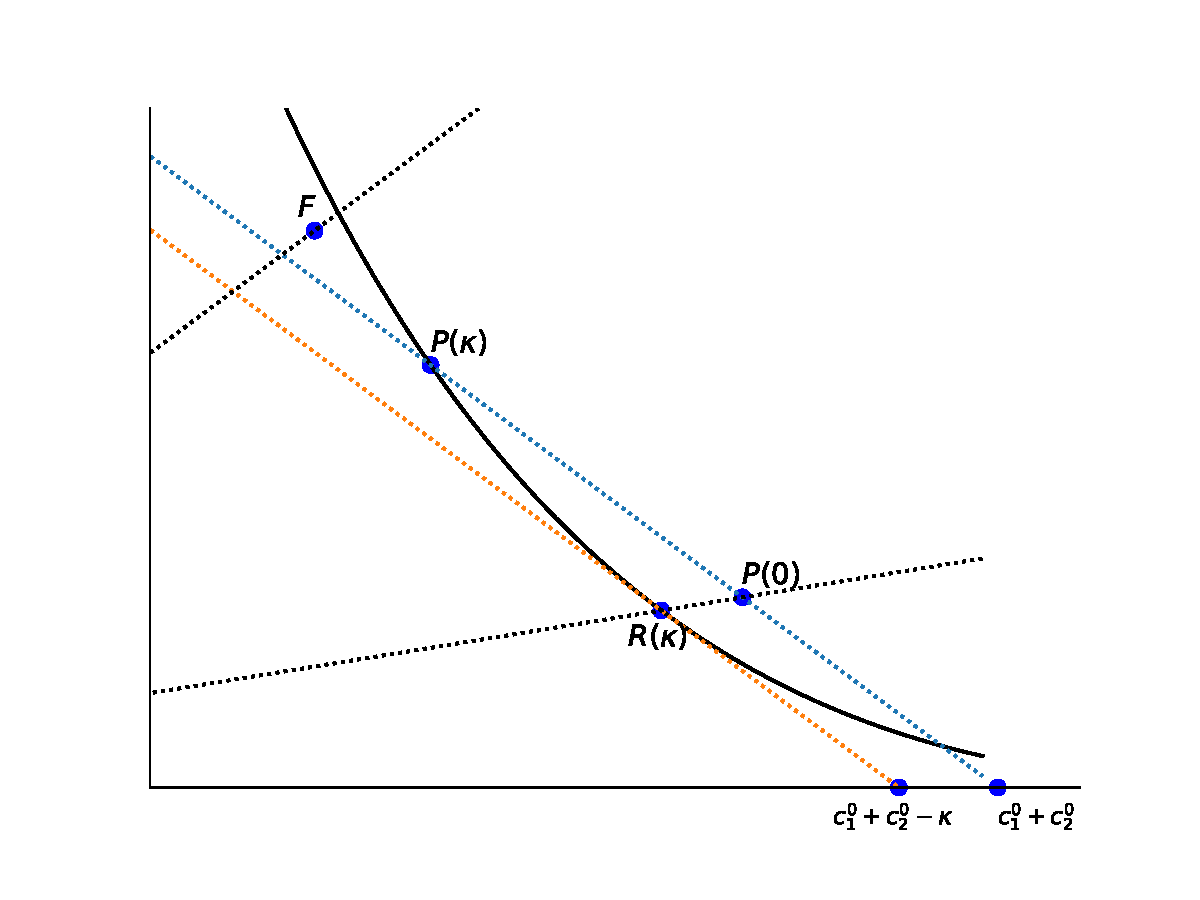
\includegraphics[width=1\textwidth]{CompetitiveRP.pdf}
  \caption{Imperfect smoothing commitment contract with $\kappa<\bar{\kappa}$}
  \label{fig:compRP} 
\end{figure}

A bank will only renegotiate away from a contract along this
budget line if the renegotiated contract $(c_{1},c_{2})$ lies on
or below iso-cost line $c_{1}+c_{2}=y-c_{0}^{0}-\kappa$. That is
because, by design, any contract above this line will not offer sufficient
cost savings (i.e. profit gain) to cover renegotiation cost $\kappa$.
Note also that candidate renegotiation contracts must satisfy One-self's
first order condition $u'(c_{1})=\beta u'(c_{2})$ \textendash{} otherwise
the gains to trade from renegotiation could be increased to make these
renegotiation more attractive. The contract that just satisfies these
two conditions is represented by point $R(\kappa)$.\footnote{With period 0 competitive we'll have $c_{1}^{0}+c_{2}^{0}=y-c_{0}^{0}$
and can therefore identify this point from $u'(c_{1})=\beta u'(y-c_{0}^{0}-\kappa-c_{1})$.
For the CRRA case $c_{1}=(y-c_{0}^{0}-\kappa)/(1+\beta^{\frac{1}{\rho}})$.}

We have drawn an indifference curve for One-self's preferences
through this point. All points along the period 1 budget line $c_{1}^{0}+c_{2}^{0}=y-c_{0}^{0}$
that also lie above this indifference curve will be renegotiation-proof
contracts. To see this consider any contract $P'$ along this segment
(or indeed any point in the half-eye). One-self will only accept renegotiation
away from this contract if it moves One-self to an indifference curve
higher than the one running through $P'$. By construction however
any such contracts must lie above the bank's no-renegotiation line
and hence would be rejected. By similar reasoning any contract along
the budget line outside of this top-segment of the half-eye would
be renegotiated. Since Zero-self's welfare increases as as we move
toward a more balanced consumption bundles, of all possible renegotiation-proof
contracts Zero prefers the contract labeled $P(\kappa)$ that offers
the highest intertemporal utility. This preferred renegotiation-proof
contract offers less consumption smoothing compared to the full-smoothing
commitment contract (reached at $\kappa\ge\bar{\kappa}$ where the
no-renegotiation constraint ceases to bind).

Mathematically, for any $c_{0}^{0}$ chosen in period 0 the
best renegotiation-proof continuation contract can be found as follows.
The Bank no-renegotiation condition $c_{1}^{1}+c_{2}^{1}=y-c_{0}^{0}-\kappa$
and the first order condition for a renegotiated contract $u(c_{1}^{1})=\beta u(c_{1}^{2})$
are used together to solve for the bank's renegotiation offer $c_{1}^{0}$
and $c_{2}^{0}$ (point $R(\kappa)$) as a function of pre-determined
$y,c_{0}^{0}$ and $\kappa$.

From One-self's no-renegotiation condition $u(c_{1}^{0})+\beta u(c_{2}^{0})=u(c_{1}^{1})+\beta u(c_{2}^{1})$
and One's first-order condition we can then solve for the optimal
continuation $c_{1}^{0}$ and $c_{2}^{0}$ as a function of those
same pre-determined variables. Using this method to find the best
continuation contract for candidate $c_{0}^{0}$ Zero-self can now
search over all candidate $c_{0}^{0}$ to find the welfare maximizing
three-period contract.

Except for the special case where $\kappa=0$, there will
be no simple closed form solution for the optimal contract even in
the CRRA case. This can be seen from the fact that there are in fact
two points where the no-renegotiation condition indifference curve
crosses the period 1 zero-profit line. As described in the appendix
for the\ CRRA\ case the $c_{1}^{0}$ coordinates of these two roots
are given by a non-linear equation (\ref{eq:no-renegotiation}).

In the special case of perfect competition with costless renegotiation
($\kappa=0$) the above equation has just one solution. In terms of
figure \ref{fig:compRP} think of how $P$ would slide down the period
1 budget line as $\kappa$ shrinks until we get to a point where One's
indifference curve is just tangent to the period 1 budget line. This
continuation contract is 'renegotiation-proof' but only in the very
narrow sense that it won't be renegotiated because it already delivers
One-self's preferred consumption choice. Being a sophisticate, Zero
understands that the only way to avoid renegotiation is to satisfy
One's period 1 first-order condition $u'(c_{1}^{0})=\beta u'(c_{2}^{0})$.
Knowing this, the optimal contract can be explicitly solved for (\ref{eq:zerokappa-comp}).

To illustrate with an example: at our earlier parameterization
$\beta=0.5$ and $\rho=1$ the full-smoothing commitment contract
will be $C_{0}^{P}=(150,100,50)$ which offers considerably less consumption
smoothing in later periods compared to the contract with self-control
$C_{0}^{F}=(150,75,75)$. If the consumer's initial income stream
were $Y_{0}=(100,100,100)$ then we could think of the consumer with
self-control as sticking to a balanced repayment program to keep consumption
steady in the last two periods. Compared to this the consumer without
self-control rolls over debt rather than repay it in period one. The
entire burden of repayment of the debt that Zero took out in period
0 now falls in period 2, whereas Zero would have preferred the burden
to be shared equally between periods 1 and 2. If the income stream
had instead been $Y_{0}=(200,50,50)$ then a consumer without self-control
would be viewed as raiding savings in period 1 that an otherwise identical
consumer with self-control would have earmarked for period 2 consumption.

In this example, consumers that can obtain full-smoothing
commitment contracts will save/repay more or borrow less in period
1 and consume more in period 2 and the inability to do so leads to
lower welfare for Zero in this competitive setting. However, this
is not generally true, as we show below. Credible division rules between
periods 1 and 2 depend on the no-renegotiation constraint in some
subtle ways.

\subsubsection{Properties of the contract}

Suppose contract $C_{0}^{P}$ is the solution to the maximization
problem described by \ref{eq:cobj0}, \ref{eq:BPC0} and \ref{eq:no-reg-monop}.
\begin{prop}
Suppose $\kappa<\bar{\kappa}$ and the consumer is sophisticated.
Under competition, the competitive renegotiation-proof contract that
maximizes Zero-self's discounted utility ($C_{0}^{P}$) has the following
properties:

(i) $U_{0}\left(C_{0}^{P}\right)<U_{0}\left(C_{0}^{F}\right)$

(ii) The relationship between $c_{0}^{P}$ and $c_{0}^{F}$ is ambiguous.
There is some $\hat{\rho}$ such that: if $\rho\leq\hat{\rho}$, then
$c_{0}^{P}>c_{0}^{F}$; if $\rho>\hat{\rho}$, then there are parameter
values under which $c_{0}^{P}<c_{0}^{F}$. 
\end{prop}
The first statement is straightforward: Since $\kappa<\bar{\kappa}$
means the new renegotiation-proofness constraint (\ref{eq:no-reg-monop})
binds full-smoothing smoothing cannot be achieved and the consumer's
welfare must be lower than under the first-best contract.

Now, will period 0 consumption be higher or lower than under full-smoothing
commitment? The proposition is that this depends on parameter values,
in particular the intertemporal elasticity of substitution $\frac{1}{\rho}$.
Consider the competitive full-smoothing commitment contract $C_{0}^{F}$.
Following the first-order condition (\ref{eq:foc-newnotation}), it
must be true that:

\[
\frac{du\left(c_{0}^{F}\right)}{dc_{0}}=\frac{\partial V\left(s^{F},\frac{1}{2}\right)}{\partial s}
\]

Now suppose the competitive renegotiation-proof contract $C_{0}^{P}$
that involves the same period 0 consumption as under full-smoothing
commitment, so that $c_{0}^{P}=c_{0}^{F}$. By the bank's zero-profit
constraint, the contract will also have $s^{P}=s^{F}$, but consumption
will be split in period 1's favor. If the utility function is relatively
linear (low $\rho$), then an imbalanced split of $s$ results in
a lower marginal utility than from a balanced split. So: 
\[
\frac{du\left(c_{0}^{F}\right)}{dc_{0}}>\frac{dV\left(s^{F},\alpha\left(s^{F}\right)\right)}{ds}
\]

In such a case, the renegotiation-proof contract must involve higher
period 0 consumption than the full-smoothing commitment contract.

If, on the other hand, the utility function is highly convex (high
$\rho$), then an imbalanced split results in higher marginal utility
relative to full-smoothing. In such cases, the renegotiation-proof
contract will have lower period 0 consumption than under full-smoothing
commitment under certain parameter values.\footnote{The precise construction of the cutoff value $\hat{\rho}$ is somewhat
complicated, as $\frac{dV}{ds}$ depends not just on $u'\left(c_{1}\right)$
and $u'\left(c_{2}\right)$, but also on how the sharing rule, $\alpha\left(s\right)$,
changes with $s$.} This can be seen more explicitly in the case of $\kappa=0$ (Equation
\ref{eq:zerokappa-comp}).

So, under competition, the renegotiation-proofness constraint could
change the contract in either direction: a larger loan (less saved)
or a smaller loan (more saved). Period 2 consumption however always
falls relative to the full-smoothing commitment case, even in the
cases when Zero saves more/borrows less. In fact for CRRA utility
the adjustment of period 0 consumption (in the absence of commitment
compared to with commitment) is always relatively small while the
adjustment to period 1 and period 2 consumption is relatively much
larger.\footnote{To illustrate, with $\kappa=0$ at no point does period 0 consumption
rise or fall by more than six percent for any value $\rho\in(0,\infty)$
and $\beta\in(0,1)$ but at reasonable parameter values such as $\rho=0.5$
and $\beta=0.5$ in the absence of commitment period 1 consumption
rises to 149 percent of the level it would be with commitment, and
period 2 consumption falls to just 37 percent of what it would be.} In other words despite having a first-mover advantage, Zero can do
little other than to partially accommodate to the consumption pattern
that One-self wants to impose.

The contrast between monopoly and competition can be explained using
the intuition of income and substitution effects. In either case,
a move from full-smoothing commitment to renegotiation-proofness can
be viewed as a rise in the ``price'' of future utility from Zero-self's
perspective. As a result, substitution effects will lead to an increase
in period 0 consumption and a drop in future consumption. Under monopoly,
since the consumer is always left at her autarky utility, there are
no income effects. When the renegotiation-proofness constraint binds,
the price of future utility effectively rises, as a result of which
substitution effects lead to greater period 0 consumption. Under competition,
income and substitution effects work against each other; the net result
depends on the shape of the consumer's utility function.

\subsection{Contracting with Naive Hyperbolic Discounters}

For naive agents, the problem of renegotiation does not generally
lead to a renegotiation-proof contract. The naif believes she will
not be tempted to renegotiate. Banks therefore offer contracts that
take into account the potential renegotiation. Under monopoly, the
bank adds to its profits by engaging in renegotiation that was not
anticipated by the consumer in period 0. Under competition, banks
return the potential surplus from renegotiation to the Zero-self.\footnote{A similar analysis could be carried out if consumers were misinformed
not about their own preferences but about $\kappa$.}

\subsubsection{Monopoly}

Relative to a sophisticated consumer, with a naive consumer the monopolist
bank can make additional profits on two margins. First, since there
is no perceived renegotiation problem, the consumer is willing to
accept a contract that is more profitable for the bank up-front; subsequently,
possible renegotiation generates additional profits for the bank.

The bank must choose between a renegotiation-proof contract and one
that will be renegotiated upon. If $\kappa$ is sufficiently large
there is little to gain from renegotiation and the consumer will be
offered the full-smoothing commitment contract. But when $\kappa$
is relatively small, the bank might prefer to offer a contract that
will subsequently be renegotiated. In such cases, the bank solves
the following problem:\footnote{We do not need to worry about a renegotiation-proofness constraint
here. Since period 0 believes her period 1 preferences are consistent
with her own, she expects any renegotiation of the period 0 contract
to yield the same discounted utility as the contract itself.} 
\begin{eqnarray}
\underset{C_{0}}{max} & \Pi_{0}\left(C_{0};Y_{0}\right)+\Pi_{1}\left(C_{1}^{m1}\left(C_{1}\right);C_{1}\right)-\kappa\nonumber \\
s.t. & U_{0}\left(C_{0}\right)\geq U_{0}^{A}\label{eq:pc-n}
\end{eqnarray}

Let the solution be denoted $C_{0}^{mN}$. This is explicitly derived
in the appendix (\ref{eq:naive-monopolist-contract1}, \ref{eq:naive-monopolist-contract2}).
As under competition, the bank maximizes profits by offering a contract
that divides future consumption as much in favor of period 2 as possible.
The greater the imbalance between the contracted $c_{1}$ and $c_{2}$,
the greater the bank's profits from renegotiation.

This contract can be compared to the full-smoothing commitment contract
and to the renegotiation-proof contract for sophisticates. In particular,
it will involve lower period 0 consumption than under full-smoothing
commitment or renegotiation-proofness. This result appears counter-intuitive.
In the case of lending, it does not reinforce the narrative of banks
preying on naive consumers by offering them relatively large loans
with steep repayments. Indeed, there are other considerations beyond
the scope of this model, such as the possibility of collateral seizure,
that could generate large loans. But our limited model helps to highlight
a particular aspect of contracting with naive hyperbolic discounters:
here, the bank offers them relatively \emph{small} loans because its
gains from renegotiation depend on the surplus that the initial contract
delivers to periods 1 and 2. In order to fully take advantage of the
consumer's naivete, the consumer must start out with sufficiently
small repayments that the bank could profit from rearranging them.

The next proposition summarizes the above discussion. 
\begin{prop}
Suppose the consumer is naive. Under monopoly:

(i) If $\kappa$ is sufficiently higher than $\bar{\kappa}^{m}$,
the firm will offer the agent the full-smoothing commitment contract
($C_{0}^{mF}$) and it will not be renegotiated. 

(ii) Otherwise, the contract $C_{0}^{mN}$ will satisfy $c_{0}^{mN}<c_{0}^{mF}<c_{0}^{mP}$
(either explicitly or in the limit), and it will be renegotiated in
period 1. 
\end{prop}

\subsubsection{Competition}

Under competition, with naive consumers contracts must account for
renegotiation to have firms continue earning zero profits. First,
note that if contracts are not exclusive, the equilibrium contract
must be identical to the full-smoothing commitment contract. This
is because the firm offering the contract in period 0 does not expect
to benefit from renegotiation, so the contract gets competed down
to the one that maximizes the naive Zero-self's perceived utility
while delivering zero profits to the bank.

Under exclusive contracts, anticipated profits from future renegotiation
will be returned to the consumer through more favorable initial contracts.
If $\kappa$ is sufficiently small, the equilibrium contract involves
renegotiation and satisfies: 
\begin{align}
\underset{C_{0}}{\mbox{\ensuremath{max}}} & U_{0}\left(C_{0}\right)\nonumber \\
s.t. & \Pi_{0}\left(C_{0};Y_{0}\right)+\Pi_{1}\left(C_{1}^{m1}\left(C_{1}\right);C_{1}\right)\geq\kappa
\end{align}

Let the solution be denoted $C_{0}^{N}$. This is explicitly derived
in the appendix (\ref{eq:naive-comp-contract1} and \ref{eq:naive-comp-contract2}).
Contracts divide future consumption as much in favor of period 2 as
possible. We show that if $\rho<1$, the contract is at a corner solution
where $c_{1}=0$. If $\rho>1$, an explicit solution does not exist,
but maximization pushes the contract to a point where $c_{2}$ approaches
infinity.\footnote{This can be dealt with by a reasonable assumption of an upper bound
on contract terms.} This maximizes the potential gains from renegotiation. In the context
of loans, this suggests contracts where the debt burden is heaviest
in the intermediate stages, resulting in renegotiation to postpone
payments.

Unlike under monopoly, these anticipated renegotiation gains must
be returned to the consumer. Some of these gains are returned to the
Zero-self, so there is no clear prediction about whether period 0
consumption will be lower or higher than under full-smoothing commitment.
\begin{prop}
Suppose the consumer is naive. Under competition:

(a) If contracts are not exclusive: The consumer will accept the full-smoothing
commitment contract, $C_{0}^{F}$. The contract will be renegotiated
in period 1 if and only if $\kappa<\bar{\kappa}$.

(b) If contracts are exclusive: 

(i) If $\kappa$ is sufficiently higher than $\bar{\kappa}$, the
consumer will accept the full-smoothing commitment contract ($C_{0}^{F}$)
and it will not be renegotiated. 

(ii) Otherwise, the consumer will accept a contract $C_{0}^{N}$ with
the following properties: if $\rho<1$, $c_{0}^{N}<c_{0}^{F}$. If
$\rho>1$, then there are parameter values under which $c_{0}^{N}>c_{0}^{F}$. 
\end{prop}

\section{Not for profit and hybrid ownership forms}\label{nonprofits}

Consider next the case of a firm that, in a pre-contract stage, has
the possibility of choosing its ownership structure say by incorporating
as a legal non-profit or, more broadly, by choosing a degree of `hybrid'
ownership, for example by retaining for-profit status but allowing
social investors to establish considerable ownership stakes and managerial
control. In the spirit of Hansmann () and the discussion in the introduction,
we model this as a restriction on the firm's ability to distribute
raw profits to managers and shareholders:
\begin{defn*}
Given `raw profits' $\Pi_{0}$, a `nonprofit' firm retains `captured
profits' $f\left(\Pi_{0}\right)$, where $f\left(0\right)=0$, $f'\left(\Pi_{0}\right)\in\left(0,1\right)$,
and $f''\left(\Pi_{0}\right)\leq0.$ 
\end{defn*}
This formulation follows \citet{glaeser2001} who
argued that though the principals of a non-profit may be technically
legally barred from tying compensation to cash profits, they can in
practice capture a fraction of those profits in costly and imperfect
ways via the consumption of perquisites or `dividends in kind' (e.g.
the lavish expense account). The ability of perquisites to substitute
for unrestricted consumption falls as profits get larger. 

Setting aside welfare concerns that might drive firms to adopt nonprofit
or hybrid status, we examine when purely profit-minded firms might
make such governance choices; i.e. when can a voluntary restriction
on the ability to enjoy profits make a self-interested firm better
off?\footnote{Indeed, welfare concerns could directly improve consumer outcomes
by either allowing Zero-self's participation constraint to be slack
or by raising the costs of renegotiation $\kappa$. We consider the
latter point in an example below.} This has parallels to the explanation for commercial nonprofits due
to \textbackslash{}cite\{hansmann\_ownership\_1996\} and modeled by
\textbackslash{}citet\{glaeser\_not-for-profit\_2001\} but is established
on different behavioral grounds.\footnote{In those accounts a firm may choose to deliver less than a promised
quantity or quality of a good or service, unambiguously harming the
time-consistent client. After the fact the client who discovers the
fact would always want to challenge the contract breach and does not
do so only because by assumption it is too difficult or costly. In
our model on the other hand the firm and the One-self customer both
gain by voluntarily breaking the existing contract commitments and
there is no Zero-self to mount a challenge.} 

At the outset, it should be noted that profit-oriented principals
have no incentive to switch to hybrid/nonprofit status when consumers
are naive. Since the consumer does not perceive a need for commitment,
any promise of superior commitment is of no value to her. The analysis
with sophisticated consumers follows.

\subsection{Monopoly}

In a pre-contract phase the firm now first establishes its type via
the adoption of legal non-profit status and/or by choosing credible
and stable ownership and governance structures that commit it to those
limitations. If the monopoly firm were to operate as a nonprofit or
a hybrid, when facing a sophisticated hyperbolic discounter it would
design a renegotiation-proof contract to solve:
\begin{align}
 & \underset{C_{0}}{max}\text{ }f\left(\Pi_{0}\left(C_{0};Y_{0}\right)\right)\\
 & U_{0}\left(C_{0}\right)\geq U_{0}^{A}\\
 & f\left(\Pi\left(C_{0};Y_{0}\right)+\Pi_{1}\left(C_{1}^{m1}\left(C_{1}\right);C_{1}\right)\right)-f\left(\Pi\left(C_{0};Y_{0}\right)\right)\leq\kappa\label{eq:no-reneg-np}
\end{align}

Why might a profit-maximizing firm choose to operate as a nonprofit
when that reduces its ability to capture profits? The answer lies
in the loosening of the no-renegotiation constraint (\ref{eq:no-reneg-np}).
Any gains from renegotiation are worth less than they would be to
the for-profit firm. Clearly, the for-profit monopolist's contract
($C_{0}^{mP})$ would now leave the no-renegotiation constraint slack.
Because the non-profit can more credibly commit to not renegotiate
contracts that offer greater consumption smoothing across periods
1 and 2, Zero-self becomes more willing to pay for this consumption
stream.

The captured-profits maximizing solution gives a contract that we
denote $C_{0}^{mNP}$. If $\kappa<\bar{\kappa}^{m}$, with a relaxed
renegotiation-proof constraint $\Pi_{0}(C_{0}^{mNP};Y_{0})>\Pi_{0}(C_{0}^{mP};Y_{0})$
but whether or not it will be in the bank principals' best interest
to strategically convert to non-profit status depends on whether the
captured profits under non-profit status exceed the profits they could
earn as a pure for-profit, in other words on whether $f\left(\Pi_{0}(C_{0}^{mNP};Y_{0})\right)>f\left(\Pi_{0}(C_{0}^{mP};Y_{0})\right)$.
The monopolist faces a tradeoff in considering non-profit status:
higher raw profits (as the commitment problem is partly solved) but
a diminished capture of those raw profits.

Does the rise in extracted surplus outweigh the fact that all profits
are now discounted? Proposition 6 (in Section 5.2) establishes the
existence of captured profit functions that would be strictly preferred
to for-profit status for monopoly firms. This is easy to see: the
possible concavity of $f$ could leave the enjoyment of profits relatively
unaffected while significantly loosening the no-renegotiation constraint
(since renegotiation would raise profits further, and since $f$ is
concave, these additional profits would count for little).

Given particular captured profit functions, we can also ask which
consumers are more likely to be served by nonprofit monopolists. If
consumers are far from optimal in autarky, then the for-profit firm
would anyway be making substantial profits. In this case, the nonprofit's
credibility advantages are not enough to outweigh the fact that it
loses a significant amount of enjoyment of its profits due to legal
restrictions. 

However, for consumers with higher autarky utility, the gains that
can be captured from nonprofit status are large relative to the profits
that a for-profit would have made, so the firm prefers to operate
as a nonprofit. As an example, consider an autarky consumption bundle
at which the for-profit firm would earn zero profits. Now, the nonprofit
firm can earn positive profits, so regardless of $f$ nonprofit status
dominates.

\subsubsection{An example}

Let us consider a situation where a firm may choose it's degree
of hybrid-ness or for-profit orientation, indexed by a parameter $\alpha\in\left[0,1\right]$.
For a chosen $\alpha$, let the captured profits function be linear:
\begin{equation}
f\left(\Pi_{0}\right)=\alpha\Pi_{0}
\end{equation}


We can interpret $\alpha$ as the maximum fraction of raw
profits that can be distributed to managers and shareholders. An $\alpha=1$
would represent a pure for-profit investor-led firm, $\alpha=0$ a
strictly regulated non-profit.

We can also allow $\alpha$ to directly affect the non-pecuniary
renegotiation cost the firm's principals incur when they opportunistically
break contractual promises to customers. A more hybrid or non-profit
firm dominated by social investors is more likely to hire staff and
managers that internalize client welfare and social investor motivations
and therefore are more likely to feel non-pecuniary costs associated
with guilt, shame or loss of reputation from breaking promises. If
we now label the cost of renegotiation $\eta\left(\alpha\right)$
\textendash{} replacing our earlier $\kappa$ \textendash{} this idea
is captured by assuming that function $\eta$ falls weakly in $\alpha$.
Putting both mechanisms together gives us modified no-renegotiation
constraint (\ref{eq:no_reneg_np}) which states that the fraction
of raw profits $\Pi_{1}$ that can be captured from renegotiating
a contract must not exceed renegotiation costs: 
\begin{equation}
\alpha\Pi_{1}(C_{1}^{m1}(C_{1});C_{1})\leq\eta(\alpha)\label{eq:no_reneg_np}
\end{equation}
If we define $\kappa(\alpha)\equiv\frac{\eta(\alpha)}{\alpha}$, this
no-renegotiation constraint can be written as

\begin{equation}
  \Pi_{1}(C_{1}^{m1}(C_{1});C_{1})\leq\kappa(\alpha)\label{eq:no-kalpha}
\end{equation}
which looks like the earlier constraint (\ref{eq:rpc-m})
except $\kappa$ is now a function of $\alpha$. The earlier renegotiation
problems were for the special case of a pure for-profit firm with
$\alpha=1$ but we can now analyze contracting, captured profits,
and client welfare at any level of $\alpha$ and ownership choices
in a strategic equilibrium. 

To the extent that the loosening of the no-renegotiation constraint
happens through the right-hand side (i.e. via term $\eta\left(\alpha\right)$,
which represents the firm's motivation to honor the initial agreement),
the firm benefits unambiguously\textendash it is able to offer better
commitment \emph{and} fully retain the added profits.

\begin{figure}
  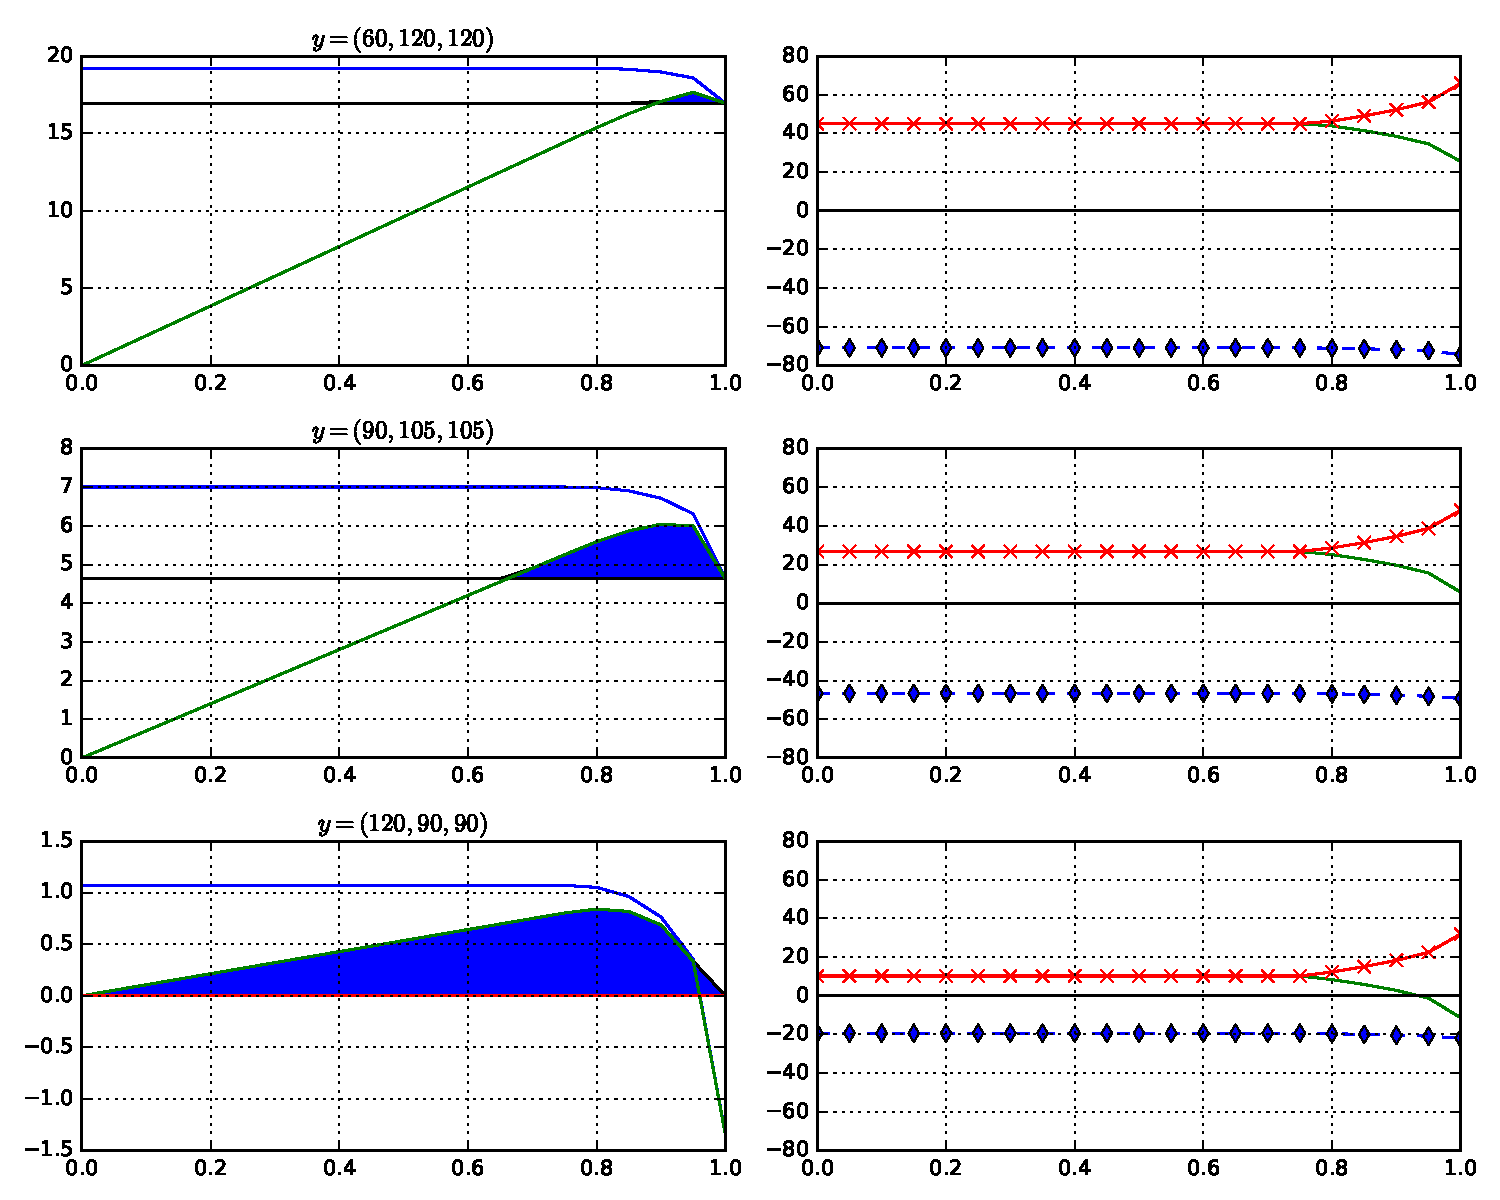
\includegraphics[width=1\textwidth]{fig_nonprofits.pdf}
  \caption{\label{fig:nonprofit}Captured rent by ownership status and endowment
income}

\end{figure}

In Figure \ref{fig:nonprofit} we illustrate the case where
non-pecuniary costs to breaking a promise not to renegotiate fall
with $\alpha$ according to $\eta(\alpha)=10(1-\alpha)$ and hence
that the overall cost to renegotiation varies with $\alpha$ according
to $\kappa(\alpha)=10(1-\alpha)/\alpha$. The plots depict captured
profits that would be achieved at different levels $\alpha$ starting
from three different initial endowment streams. These three streams
- (60, 120, 120), (90, 105, 105) and (120, 90, 90) \textendash{} are
equal in their present value of 300 but differ in terms of period
0 income (with remaining income allocated equally across period 1
and 2). The higher of the two curved lines represents `raw' profits
$\Pi_{0}(C_{0}^{m\alpha};Y_{0})$ and the lower curve captured profits
$\alpha\Pi_{0}(C_{0}^{m\alpha};Y_{0})$. A horizontal line has been
drawn in to indicate the level of profits $\Pi_{0}(C_{0}^{mP};Y_{0})$
captured by a pure for-profit ($\alpha=1$). Consider the top panel
where the customer has initial income $(60,120,120)$. As this type
of customer wants to borrow heavily in period 0 profits to the bank
are large, even in the case of renegotiation-proof contracts. Adopting
non-profit status by lowering $\alpha$ confers limited profit gain
however: the cost of lowering alpha (giving up a share of already
high profits) is not compensated for by the gains from being able
to credibly commit to a smoother contract. However at $(90,105,105)$
the tradeoff is different and profits can be increased. In the picture
any non-profit with an $\alpha$ between approximately 0.7 and less
than one captures more profits than a pure for-profit. Finally for
customers with an endowment $(120,90,90)$ are already fairly close
to their preferred consumption stream so the profits to be captured
even under full commitment are not that large. Indeed in this case
a pure for-profit cannot earn positive profits. Here the cost of adopting
non-profit status is low compared to the gains, and we the simulation
reveal that any non-profit status firm captures more profits than
a pure for-profit, and maximum captured profits are achieved at around
$\alpha=0.7$.

\subsection{Competition}

\subsubsection{Exclusive contracts}

Consider what would happen in the competitive market situation now
if contracts can be assumed to remain exclusive, so that any new surplus
in the event of a renegotiation between the bank and the One-self
goes to the bank (this grants the bank monopoly power in period 1).
In this setting, a nonprofit/hybrid firm will be led to offer contract
terms to solve:
\begin{align}
\underset{C_{0}}{max} & U_{0}\left(C_{0}\right)\\
s.t. & f\left(\Pi_{0}(C_{0};Y_{0})\right)\geq0\\
 & f\left(\Pi\left(C_{0};Y_{0}\right)+\Pi_{1}\left(C_{1}^{m1}\left(C_{1}\right);C_{1}\right)\right)-f\left(\Pi\left(C_{0};Y_{0}\right)\right)\leq\kappa\label{eq:no-reneg-enp}
\end{align}

Let the contract that solves this program be denoted $C_{0}^{eNP}$
. Consider first a field where all firms start as pure for-profits
and earn zero profits. If the no-renegotiation constraint binds, Zero-self's
utility must be lower than optimal. Starting from this situation consider
now one firm's strategic choice of whether to adopt non-profit status.
One firm deviating into nonprofit status in this way can make positive
profits while offering Zero-self a contract with a higher discounted
utility because of the loosened no-renegotiation constraint (\ref{eq:no-reneg-enp}).
So, if the borrowers are sophisticated hyperbolics, in equilibrium
all firms become nonprofit. In equilibrium, firms will therefore operate
as nonprofits and earn zero profits.

\subsubsection{Non-Exclusive Contracts}

Now, assume that exclusivity and period 1 monopoly power disappears.
Firms can compete to renegotiate each other's contracts in period
1.

If there were only nonprofits in equilibrium, any one firm could make
positive profits by switching to for-profit status and undoing a rival
bank's contract in period 1. The advantages of undercutting other
firms' contracts outweigh the benefits of promising one's own clients
it will not renegotiate. As a result, equilibrium contracts will be
determined by for-profit firms, and consumers will be offered lower
commitment than from non-profit firms alone.\footnote{The same argument applies if banks can costlessly renegotiate other
bank's contracts.} Additionally, a smaller range of consumer types will be serviced
relative to the case with exclusive contracts. 

The above discussion is summarized in the following proposition.
\begin{prop}
(a) Suppose $\kappa<\bar{\kappa}^{m}$. Under monopoly, there exist
captured profit functions such that the firm will operate as a nonprofit.

(b) Suppose $\kappa<\bar{\kappa}$. Under competition: (i) If contracts
are exclusive, firms will operate as nonprofits for any captured profit
discount function. (ii) If contracts are not exclusive, there is no
captured profit discount function under which firms will operate as
nonprofits.
\end{prop}

\section{Additional considerations}\label{considerations}

Our preceding analysis made the simplifying assumption that contracts
between consumers and banks could only be initiated in period 0. The
alternative to a period 0 contract was autarky for the consumer and
zero profits for the bank. This served to streamline the analysis.
We now discuss the interesting problem of how the contract space is
enriched by allowing unbanked consumers to sign two-period contracts
in period 1, possibly without contracting in period 0.\footnote{We thank Abhijit Banerjee for helpful discussions on this point.}
The main change will relate to the formulation of reservation values
and their implications for the shape and feasibility of the period
0 contracts. This does not change most qualitative results of the
paper but the discussion raises interesting questions about circumstances
where consumers could be better off under an autarky economy compared
to one with a financial intermediary.

Consider the monopolist bank facing a sophisticated hyperbolic discounter.
If a contract were not signed in period 0, they would meet again in
period 1. In period 1, the contract must satisfy One-self's participation
constraint, which would be determined by some unbanked consumption
path $C_{1}^{A'}$. This can be stated formally. Given some consumption
path $C_{1}^{A'}$, the bank solves: 
\begin{align*}
\underset{C_{1}}{\max}\text{ }{\Pi_{1}\left(C_{1};C_{1}^{A'}\right)}\\
\text{s.t. }U_{1}\left(C_{1}\right)\geq U_{1}\left(C_{1}^{A'}\right)
\end{align*}

Let the solution be denoted $C_{1}^{m'}$. Two observations can be
made. First, the bank can always offer a period 1 contract that delivers
nonnegative profits. This is because any contract will satisfy One-self's
optimality condition, $u'\left(c_{1}^{m'}\right)=\beta u'\left(c_{2}^{m'}\right)$.
So, except in the special case where the autarky consumption path
satisfies this condition, the bank can make positive profits in period
1. Second, the autarky consumption path $C_{1}^{A'}$ might differ
from $C_{1}^{A}$, the consumer's autarky utility in the absence of
banking. In other words, $C_{1}^{A}$ maximizes $U_{0}\left(C_{0}^{A}\right)$
while $C_{1}^{A'}$ maximizes $U_{0}\left(c_{0}^{A'},c_{1}^{m'},c_{2}^{m'}\right)$.
In the latter case, period 0 anticipates that consumption across periods
1 and 2 is guaranteed to satisfy period 1's optimality condition.
We can denote $C_{0}^{B}\equiv\left(c_{0}^{A'},c_{1}^{m'},c_{2}^{m'}\right)$,
which corresponds to a Zero-self utility of $U_{0}^{B}$.

In period 0, any contract must meet the Zero-self's reservation utility,
$U_{0}^{B}$: 
\begin{align*}
\underset{C_{0}}{max} & \Pi_{0}\left(C_{0};Y_{0}\right)\\
\text{s.t.} & \text{\ensuremath{U_{0}\left(C_{0}\right)\geq U_{0}^{B}}}
\end{align*}

The maximization problem looks familiar, apart from the modified reservation
utility. The Zero-self's discounted utility from such a contract is
no longer monotonic in her Zero-self's full-autarky utility, $U_{0}^{A}$.
For example, consider two hypothetical consumers who in autarky must
consume their income streams, which deliver the same autarky utility
but through different consumption paths: consumer X has $c_{1}^{A}=c_{2}^{A}$
while consumer Y has $c_{1}^{A}>c_{2}^{A}$ in a way that satisfies
period 1's optimality condition. Then, for consumer X, $U_{0}^{B}<U_{0}^{A}$
while for consumer Y, $U_{0}^{B}=U_{0}^{A}$. It follows that, since
period 0 contracts depend on the distribution of future consumption,
a consumer who fares relatively better in the absence of a bank may
fare relatively worse under a banking contract.

Given this benchmark full-commitment contract, the renegotiation-proof
contract can be solved for by adding a no-renegotiation constraint
to the above maximization problem. The constraint is the same as used
previously, and again narrows the set of contracts that can be offered
in period 0. As in Proposition 2, the renegotiation-proof constraint
results in lower profits and greater period 0 consumption relative
to full-commitment. These results are independent of the period 0
reservation utility and therefore remain unchanged.

A key difference here, however, is that a renegotiation-proof contract
will be offered to all consumers (unlike before, where the bank was
better off not contracting with consumers whose autarky utility left
them close enough to the first-best). Intuitively, this is because
the alternative to a period 0 contract is not autarky; rather, it
is a period 1 contract that tilts consumption in period 1's favor.
Since, in period 0, the bank can at least offer the consumer a consumption
path of $C_{0}^{B}$, it ensures that a contract will be accepted.

By opening up the possibility of period 1 contracts, we introduce
an additional consideration\textendash the same bank that offers commitment
itself creates a need for commitment. By threatening to fully indulge
the One-self's preferences, the bank is always able to induce the
Zero-self to accept an offer of partial commitment, no matter how
weak.

Finally, observe that the bank's decision about whether to operate
as a nonprofit is subject to the same tradeoff between improved commitment
and reduced enjoyment of profits. However, under monopoly the attractiveness
of nonprofit status drops (relative to the case where period 1 contracts
are disallowed) due to the fact that even the for-profit bank finds
it profitable to offer contracts to consumers at all levels of autarky
utility.

\section{Conclusion}

The starting point for this paper is the observation that the solution
to any commitment problem must also address a renegotiation problem.
We show how the renegotiation problem depends on costs of renegotiation
and how it changes contract terms in sometimes unexpected ways. In
this context, we also provide a rationalization of commercial nonprofits
in the absence of asymmetric information.

We argue that the model sheds some light on trends in microfinance,
payday lending, and mortgage lending. We hope this paper also offers
a framework that can be built upon. The incorporation of additional
`real-world' factors could improve our understanding of particular
institutions and generate empirically relevant comparative statics.
Examples of these include nondeterministic incomes, private and heterogenous
types, collateral and strategic default, and longer time horizons.

Furthermore, the analysis could be expanded to heterogeneous populations.
For instance, how might a monopoly's governance choices be affected
when it serves a market that comprises both naive and sophisticated
hyperbolic discounters? With sophisticates, the firm would prefer
high renegotiation costs while with sophisticates, it would prefer
that the same costs be low.

Finally, the differences between monopoly and competition open up
some new, potentially interesting questions. How does market structure
evolve and what are the implications for commitment? And through this
evolution might there emerge third parties to contracts between consumers
and banks that can more effectively enforce the commitment that is
sought after on both sides of the market?

\section{Appendix: CRRA Derivations and Proofs}

\subsection{Full-commitment}

\subsubsection{Competition}

Combining the first-order conditions (\ref{eq:FOC_comp}) and the
budget constraint (\ref{eq:BPC0}) of the utility maximization problem,
the competitive full-smoothing commitment contract $C_{0}^{F}$ is:
\begin{equation}
C_{0}^{F}=\left(\frac{y}{1+2\beta^{\frac{1}{\rho}}}\right)\cdot\left(1,\beta^{\frac{1}{\rho}},\beta^{\frac{1}{\rho}}\right)\label{eq:c-f}
\end{equation}

\subsubsection{Monopoly}

For the monopolist bank that offers full-commitment, the solution
is determined by the first-order condition and the consumer's participation
constraint: 
\begin{align}
C_{0}^{mF} & =\left(\frac{U_{0}^{A}\left(1-\rho\right)}{1+2\beta^{\frac{1}{\rho}}}\right)^{\frac{1}{1-\rho}}\cdot\left(1,\beta^{\frac{1}{\rho}},\beta^{\frac{1}{\rho}}\right)\label{eq:c-mf}\\
\Pi_{0}\left(C_{0}^{mF};Y_{0}\right) & =y-\left(U_{0}^{A}\left(1-\rho\right)\right)^{\frac{1}{1-\rho}}\left(1+2\beta^{\frac{1}{\rho}}\right)^{\frac{-\rho}{1-\rho}}\label{eq:pi-mf}
\end{align}

It can easily be verified that $C_{0}^{F}>C_{0}^{mF}$.

\subsection{Renegotiation }

\subsubsection{Renegotiated contracts}

Given an existing continuation contract $C_{1}^{0}$ , assuming the
contract is renegotiated, the competitively renegotiated contract
will be: 
\begin{equation}
C_{1}^{1}\left(C_{1}^{0}\right)=\left(\frac{c_{1}^{0}+c_{2}^{0}-\kappa}{1+\beta^{\frac{1}{\rho}}}\right)\cdot\left(1,\beta^{\frac{1}{\rho}}\right)\label{eq:c-r}
\end{equation}

And under monopoly, the renegotiated contract will be: 
\begin{equation}
C_{1}^{m1}\left(C_{1}^{0}\right)=\left(\frac{(c_{1}^{0})^{1-\rho}+\beta(c_{2}^{0})^{1-\rho}}{1+\beta^{\frac{1}{\rho}}}\right)^{\frac{1}{1-\rho}}\cdot\left(1,\beta^{\frac{1}{\rho}}\right)\label{eq:m-r}
\end{equation}

The corresponding profit gains from renegotiation under monopoly are:
\begin{equation}
\Pi_{1}\left(C_{1}^{m1}\left(C_{1}^{0}\right);C_{1}^{0}\right)=\left(c_{1}^{0}+c_{2}^{0}\right)-\left((c_{1}^{0})^{1-\rho}+\beta(c_{2}^{0})^{1-\rho}\right)^{\frac{1}{1-\rho}}\left(1+\beta^{\frac{1}{\rho}}\right)^{\frac{-\rho}{1-\rho}}\label{eq:pi-r}
\end{equation}

\subsubsection{No-renegotiation condition}

Substituting from \ref{eq:pi-r} in the no-renegotiation condition
(\ref{eq:no-reg-monop}), we get the following explicit no-renegotiation
condition: 
\begin{align}
\Pi_{1}\left(C_{1}^{m1}\left(C_{1}^{0}\right);C_{1}^{0}\right) & =\kappa\nonumber \\
\Longleftrightarrow\left(c_{1}^{0}+c_{2}^{0}\right)-\left((c_{1}^{0})^{1-\rho}+\beta(c_{2}^{0})^{1-\rho}\right)^{\frac{1}{1-\rho}}\left(1+\beta^{\frac{1}{\rho}}\right)^{\frac{-\rho}{1-\rho}} & \leq\kappa\label{eq:no-renegotiation}
\end{align}

This condition applies identically whether contract renegotiation
happens under competition or monopoly.

\subsubsection{No-renegotiation condition for full-smoothing contracts}

Setting $c_{1}^{0}=c_{2}^{0}$ in the no-renegotiation constraint
above, we get the following simplified condition that must be satisfied
by any contract that specifies equal consumption in periods 1 and
2:
\begin{equation}
\kappa\geq c_{1}^{0}\cdotp\Upsilon\label{eq:smoothing-no-renegotiation}
\end{equation}

where
\begin{equation}
\Upsilon=\left[2-\left[\frac{(1+\beta)}{\left(1+\beta^{\frac{1}{\rho}}\right)^{\rho}}\right]^{\frac{1}{1-\rho}}\right]\label{eq:upsilon}
\end{equation}

\subsection{Imperfect-Smoothing Commitment Contracts}

Redefine any consumption stream in the following manner:
\begin{equation}
C_{0}=\left(c_{0},c_{1},c_{2}\right)\equiv\left(c_{0},\alpha s,\left(1-\alpha\right)s\right)\label{eq:new-notation}
\end{equation}
so that $c_{1}$ and $c_{2}$ are expressed as shares of total future
consumption $s$. Since the no-renegotiation constraint places restrictions
on the relative values of $c_{1}$ and $c_{2}$, we can rewrite the
constraint (\ref{eq:no-renegotiation} using the new notation to get
a continuous function $\alpha\left(s\right)$, which determines the
mimimum fraction of any $s$ that must be offered to One-self to prevent
renegotiation:
\begin{equation}
\left(s\right)\left(1-\left(\alpha^{1-\rho}+\beta\left(1-\alpha\right)^{1-\rho}\right)^{\frac{1}{1-\rho}}\left(1+\beta^{\frac{1}{\rho}}\right)^{\frac{-\rho}{1-\rho}}\right)\leq\kappa\label{eq:no-renegotiation-alpha-s}
\end{equation}

Observe that at One-self's optimal division of $s$, $\left(c_{2}=\beta^{\frac{1}{\rho}}c_{1}\Longleftrightarrow\alpha=\frac{1}{1+\beta^{\frac{1}{\rho}}}\right)$
, there cannot be profit gains from renegotiation so the constraint
will be slack. For any $s$, there may be two values of $\alpha$
that satisfy the constraint with equality\textendash one with $\alpha$
smaller than One-self would like (lower boundary), and another with
$\alpha$ larger than One-self would like (upper boundary). Assuming
the full-smoothing contract does not satisfy the constraint, the second-best
contract must lie on the lower boundary. This defines a continuous
function $\alpha\left(s\right)$, which determines the mimimum fraction
of any $s$ that must be offered to One-self to prevent renegotiation.
\begin{equation}
\alpha\left(s\right)=min\left\{ \alpha:\left(s\right)\left(1-\left(\alpha^{1-\rho}+\beta\left(1-\alpha\right)^{1-\rho}\right)^{\frac{1}{1-\rho}}\left(1+\beta^{\frac{1}{\rho}}\right)^{\frac{-\rho}{1-\rho}}\right)=\kappa\right\} \label{eq:alpha-1}
\end{equation}

It can easily be verified that $\alpha'\left(s\right)>0$ (profits
from renegotiation rise in $s$, so if $s$ rises there must be an
increase in the share allocated to 1-self to compensate). Implicitly
differentiating the binding no-renegotiation constraint by $s$, we
have:
\begin{equation}
\frac{d\alpha}{ds}=\left(\frac{k}{s^{2}}\right)\left(\frac{1+\beta^{\frac{1}{\rho}}}{\alpha^{1-\rho}+\beta\left(1-\alpha\right)^{1-\rho}}\right)^{\frac{\rho}{1-\rho}}\left(\frac{1}{\alpha^{-\rho}-\beta\left(1-\alpha\right)^{-\rho}}\right)\label{eq:dalpha-ds}
\end{equation}

The terms in the first two sets of parentheses are always positive.
The last term is positive when the no-renegotiation constraint is
binding (One-self would ideally like $\alpha^{-\rho}=\beta\left(1-\alpha\right)^{-\rho}$
but if $\kappa>0$ she has to settle for $\alpha^{-\rho}>\beta\left(1-\alpha\right)^{-\rho}$.

Finally, for any $s$ and $\alpha$, let 
\begin{equation}
V\left(s,\alpha\right)\equiv\beta\left[u\left(\alpha s\right)+u\left(\left(1-\alpha\right)s\right)\right]\label{eq:cont-utility}
\end{equation}
 This is the discounted utility over periods 1 and 2, from period
0's perspective. It will be useful to note that the first-order conditions
of the full-smoothing contract problems (competition and monopoly)
can be written as:
\begin{equation}
\frac{du\left(c_{0}\right)}{dc_{0}}=\frac{dV\left(s,\frac{1}{2}\right)}{ds}\label{eq:FOC-with-V}
\end{equation}

\subsubsection{Sophisticated Hyperbolic Discounters}

\textit{Proof of Proposition 2:} (i) Since the full-commitment
profit-maximizing contract was uniquely determined, and since it does
not satisfy the renegotiation-proofness constraint, the renegotiation-proof
contract must yield lower profits than the full-commitment contract
does.

(ii) Using the modified notation, the full-smoothing contract terms
are $c_{0}^{mF}$ and $s^{mF}$, with $\alpha^{mF}=\frac{1}{2}$.
The imperfect-smoothing contract terms are $c_{0}^{mP}$ and $s^{mP}$,
with $\alpha^{mP}=\alpha\left(s^{mP}\right)$. Suppose $c_{0}^{mP}\leq c_{0}^{mF}$.
Then, to satisfy Zero-self's participation constraint,
\begin{align}
V\left(s^{mP},\alpha\left(s^{mP}\right)\right) & \geq V\left(s^{mF},\frac{1}{2}\right)\\
\Rightarrow s^{mP} & \geq s^{mF}\left[\frac{\left(\frac{1}{2}\right)^{1-\rho}+\left(\frac{1}{2}\right)^{1-\rho}}{\left(\alpha^{mP}\right)^{1-\rho}+\left(1-\alpha^{mP}\right)^{1-\rho}}\right]^{\frac{1}{1-\rho}}\label{eq:s-compare}
\end{align}

Differentiating $V\left(s^{mP},\alpha^{mP}\right)$, we get the following
inequalities:\footnote{An explanation of the steps: Line \ref{eq:deriv2} follows from the
fact that $\alpha\left(s\right)$ rises in $s$ (derived from Equation
\ref{eq:alpha-1}) and $V$ falls as $\alpha$ rises, making the allocation
worse from Zero-self's perspective. Line \ref{eq:deriv4} follows
from Inequality \ref{eq:s-compare}. Line \ref{eq:deriv8} follows
from the FOC of the monopolist's profit-maximization problem with
full-smoothing contracts. }
\begin{align}
\frac{dV\left(s^{mP},\alpha^{mP}\right)}{ds} & =\frac{\partial V\left(s^{mP},\alpha^{mP}\right)}{\partial s}+\frac{\partial V\left(s^{mP},\alpha^{mP}\right)}{\partial\alpha}\frac{d\alpha^{mP}}{ds}\label{eq:deriv1}\\
 & <\frac{\partial V\left(s^{mP},\alpha^{mP}\right)}{\partial s}\label{eq:deriv2}\\
 & =\beta\left(s^{mP}\right)^{-\rho}\left[\left(\alpha^{mP}\right)^{1-\rho}+\left(1-\alpha^{mP}\right)^{1-\rho}\right]\label{eq:deriv3}\\
 & \leq\beta\left(s^{mF}\right)^{-\rho}\left[\frac{\left(\frac{1}{2}\right)^{1-\rho}+\left(\frac{1}{2}\right)^{1-\rho}}{\left(\alpha^{mP}\right)^{1-\rho}+\left(1-\alpha^{mP}\right)^{1-\rho}}\right]^{\frac{-\rho}{1-\rho}}\left[\left(\alpha^{mP}\right)^{1-\rho}+\left(1-\alpha^{mP}\right)^{1-\rho}\right]\label{eq:deriv4}\\
 & =\beta\left(s^{mF}\right)^{-\rho}\left[\left(\frac{1}{2}\right)^{1-\rho}+\left(\frac{1}{2}\right)^{1-\rho}\right]\left[\frac{\left(\alpha^{mP}\right)^{1-\rho}+\left(1-\alpha^{mP}\right)^{1-\rho}}{\left(\frac{1}{2}\right)^{1-\rho}+\left(\frac{1}{2}\right)^{1-\rho}}\right]^{\frac{1}{1-\rho}}\label{eq:deriv5}\\
 & <\beta\left(s^{mF}\right)^{-\rho}\left[\left(\frac{1}{2}\right)^{1-\rho}+\left(\frac{1}{2}\right)^{1-\rho}\right]\label{eq:deriv6}\\
 & =\frac{dV\left(s^{mF},\alpha^{mF}\right)}{ds}\label{eq:deriv7}\\
 & =\frac{du\left(c_{0}^{mF}\right)}{dc_{0}^{mF}}\label{eq:deriv8}\\
 & \leq\frac{du\left(c_{0}^{mP}\right)}{dc_{0}^{mP}}\label{eq:deriv9}
\end{align}

Since $\frac{dV\left(s^{mP},\alpha^{mP}\right)}{ds}<\frac{du\left(c_{0}^{mP}\right)}{dc_{0}^{mP}}$,
this contract cannot be profit maximizing for the monopolist (it could
do better by reallocating consumption away towards Zero-self). This
contradiction implies that our assumption is incorrect. It must be
true that at the profit-maximizing imperfect-smoothing contract, $c_{0}^{mP}>c_{0}^{mF}$.
$\Square$

\emph{Proof of Proposition 3:} (i) We know that $U_{0}\left(C_{0}^{F}\right)=U_{0}^{F}$.
By assumption, since the renegotiation-proofness constraint is binding,
the renegotiation-proof contract cannot offer the optimal consumption
path. Therefore $U_{0}\left(C_{0}^{P}\right)<U_{0}\left(C_{0}^{F}\right)$.

(ii) At the full-commitment contract: 
\begin{equation}
\frac{du\left(c_{0}^{F}\right)}{dc_{0}}=\frac{dV\left(s^{F},\frac{1}{2}\right)}{ds}=\left(s^{F}\right)^{-\rho}\left(2\left(\frac{1}{2}\right)^{1-\rho}\right)
\end{equation}
Consider a renegotiation-proof contract with $c_{0}=c_{0}^{F}$. To
keep bank profits zero, this contract would also have $s=s^{F}$.
But in the renegotiation-proof contract, $s$ must be divided according
to $\alpha\left(s^{F}\right)$. So: 
\begin{align}
\frac{dV\left(s^{F},\alpha\left(s^{F}\right)\right)}{ds} & =\left(s^{F}\right)^{-\rho}\left(\alpha\left(s^{F}\right)^{1-\rho}+\left(1-\alpha\left(s^{F}\right)\right)^{1-\rho}\right)\nonumber \\
 & +\frac{d\alpha\left(s^{F}\right)}{ds}\left(s^{F}\right)^{1-\rho}\left(\alpha\left(s^{F}\right)^{-\rho}-\left(1-\alpha\left(s^{F}\right)\right)^{-\rho}\right)\label{eq:dv-ds-comp}
\end{align}
The first term\textendash the direct effect of a change in $s$\textendash is
weakly less than $\frac{dV\left(s^{F},\frac{1}{2}\right)}{ds}$ if
$\rho\leq1$ and strictly greater if $\rho>1$. The second term\textendash the
component of $\frac{dV}{ds}$ that is driven by the change in $\alpha$\textendash is
strictly negative. Therefore, if $\rho<1$, $\frac{dV\left(s^{F},\alpha\left(s^{F}\right)\right)}{ds}<\frac{dV\left(s^{F},\frac{1}{2}\right)}{ds}=\frac{du\left(c_{0}^{F}\right)}{dc}$,
so the renegotiation-proof contract must satisfy $c_{0}^{P}>c_{0}^{F}$.

Next, we consider the case when $\rho>1$. We can make the following
observations about $\alpha\left(s\right)$. First, $\underset{\kappa\rightarrow0}{lim}\alpha\left(s\right)=\frac{\beta^{\frac{-1}{\rho}}}{1+\beta^{\frac{-1}{\rho}}}$.
Second, implicitly differentiating equation \ref{eq:no-renegotiation-alpha-s}
with respect to $s$, and combining it with the previous limit result,
we get $\underset{\kappa\rightarrow0}{lim}\frac{d\alpha\left(s\right)}{ds}=0$.
Therefore, if $\rho>1$ and $\kappa$ is small enough, the second
term in Equation \ref{eq:dv-ds-comp} will be sufficiently small in
magnitude that $\frac{dV\left(s^{F},\alpha\left(s^{F}\right)\right)}{ds}>\frac{dV\left(s^{F},\frac{1}{2}\right)}{ds}=\frac{du\left(c_{0}^{F}\right)}{dc}$.
In this case, the renegotiation-proof contract must satisfy $c_{0}^{P}<c_{0}^{F}$.
$\Square$

If $\kappa=0$, the renegotiation-proof contracts can be explicitly
derived since in any contract it must be true that $c_{2}=\beta^{\frac{1}{\rho}}c_{1}$.
Solving the respective maximization problems, we get the following
equilibrium contracts for monopoly and competition, respectively:
\begin{align}
C_{0}^{mP}= & \left(\left(\frac{U_{0}^{A}\left(1-\rho\right)}{1+\beta^{\frac{1}{\rho}}\left(\frac{\left(1+\beta^{\frac{1-\rho}{\rho}}\right)^{\frac{1}{\rho}}}{\left(1+\beta^{\frac{1}{\rho}}\right)^{\frac{1-\rho}{\rho}}}\right)}\right)^{\frac{1}{1-\rho}},\left(\frac{\beta+\beta^{\frac{1}{\rho}}}{1+\beta^{\frac{1}{\rho}}}\right)^{\frac{1}{\rho}}c_{0}^{mP},\beta^{\frac{1}{\rho}}\left(\frac{\beta+\beta^{\frac{1}{\rho}}}{1+\beta^{\frac{1}{\rho}}}\right)^{\frac{1}{\rho}}c_{0}^{mP}\right)\label{eq:zerokappa-monop}\\
C_{0}^{P}= & \left(\frac{y}{1+\beta+\beta^{\frac{1}{\rho}}},\left(\frac{\beta+\beta^{\frac{1}{\rho}}}{1+\beta^{\frac{1}{\rho}}}\right)c_{0}^{P},\beta^{\frac{1}{\rho}}\left(\frac{\beta+\beta^{\frac{1}{\rho}}}{1+\beta^{\frac{1}{\rho}}}\right)c_{0}^{P}\right)\label{eq:zerokappa-comp}
\end{align}

It can easily be established that $c_{0}^{mP}>c_{0}^{mF}$, $c_{0}^{P}>c_{0}^{mF}$
if $\rho>1$, and $c_{0}^{P}<c_{0}^{mF}$ if $\rho<1$.

\subsubsection{Naive Hyperbolic Discounters}

Suppose the monopolist intends to renegotiate the contract. The maximization
problem, combined with the expression for $C_{1}^{m1}\left(C_{1}\right)$
(\ref{eq:m-r}), simplifies to:

\begin{align}
\underset{c_{0},c_{1},c_{2}}{max} & y-c_{0}-\frac{\left(c_{1}^{1-\rho}+\beta c_{2}^{1-\rho}\right)^{\frac{1}{1-\rho}}}{\left(1+\beta^{\frac{1}{\rho}}\right)^{\frac{\rho}{1-\rho}}}-\kappa\\
s.t. & \frac{c_{0}^{1-\rho}}{1-\rho}+\beta\frac{c_{1}^{1-\rho}}{1-\rho}+\beta\frac{c_{2}^{1-\rho}}{1-\rho}\geq U_{0}^{A}
\end{align}

The partial derivatives of the resulting Lagrangian are: 
\begin{align}
\frac{\partial\mathcal{L}}{\partial c_{0}} & =-1-\lambda c_{0}^{-\rho}\label{eq:L0}\\
\frac{\partial\mathcal{L}}{\partial c_{1}} & =c_{1}^{-\rho}\left[-\left(\frac{c_{1}^{1-\rho}+\beta c_{2}^{1-\rho}}{1+\beta^{\frac{1}{\rho}}}\right)^{\frac{\rho}{1-\rho}}-\lambda\beta\right]\label{eq:L1}\\
\frac{\partial\mathcal{L}}{\partial c_{2}} & =c_{2}^{-\rho}\left[-\beta\left(\frac{c_{1}^{1-\rho}+\beta c_{2}^{1-\rho}}{1+\beta^{\frac{1}{\rho}}}\right)^{\frac{\rho}{1-\rho}}-\lambda\beta\right]\label{eq:L2}
\end{align}

An interior solution, with $\frac{\partial\mathcal{L}}{\partial c_{1}}=0$
and $\frac{\partial\mathcal{L}}{\partial c_{2}}=0$ does not exist
(on a $c_{1}-c_{2}$ plot, the two first-order conditions do not intersect).
If $\rho<1$, the Lagrangian is maximized at a corner solution with
$c_{1}=0$. If $\rho>1$, the Lagrangian is maximized at the limit
as $c_{2}$ approaches infinity. Using this, the maximization problem
can be re-solved. If $\rho<1$: 
\begin{equation}
C_{0}^{mN}=\left(\left(\frac{U_{0}^{A}\left(1-\rho\right)}{2+\beta^{\frac{1}{\rho}}}\right)^{\frac{1}{1-\rho}},0,\left(\frac{1+\beta^{\frac{1}{\rho}}}{\beta}\right)^{\frac{1}{1-\rho}}\left(\frac{U_{0}^{A}\left(1-\rho\right)}{2+\beta^{\frac{1}{\rho}}}\right)^{\frac{1}{1-\rho}}\right)\label{eq:naive-monopolist-contract1}
\end{equation}
If $\rho>1$, the solution is undefined, but in the limit is given
by: 
\begin{equation}
C_{0}^{mN}=\left(\left(\frac{U_{0}^{A}\left(1-\rho\right)}{1+\left(1+\beta^{\frac{1}{\rho}}\right)\beta^{\frac{1}{\rho}}}\right)^{\frac{1}{1-\rho}},\beta^{\frac{1}{\rho}}\left(1+\beta^{\frac{1}{\rho}}\right)^{\frac{1}{1-\rho}}\left(\frac{U_{0}^{A}\left(1-\rho\right)}{1+\left(1+\beta^{\frac{1}{\rho}}\right)\beta^{\frac{1}{\rho}}}\right)^{\frac{1}{1-\rho}},\infty\right)\label{eq:naive-monopolist-contract2}
\end{equation}

Let us define profits from such a contract as: 
\[
\Pi_{0}^{mN}\equiv\Pi\left(C_{0}^{mN};Y_{0}\right)+\Pi_{1}\left(C_{1}^{m1}\left(C_{1}^{mN}\right);C_{1}^{mN}\right)-\kappa
\]

\emph{Proof of Proposition 4:} (i) and (ii) are simultaneously
established through the following observations. First, $\Pi_{0}^{mN}$
is strictly falling in $\kappa$ while $\Pi_{0}\left(C_{0}^{mF};Y_{0}\right)$
is invariant in $\kappa$. Second, at $\kappa=\bar{\kappa}^{m}$,
\begin{equation}
\Pi_{0}\left(C_{0}^{mF};Y_{0}\right)=\Pi_{0}\left(C_{0}^{mF};Y_{0}\right)+\Pi_{1}\left(C_{1}^{m1}\left(C_{1}^{mF}\right);C_{1}^{mF}\right)-\kappa<\Pi_{0}^{mN}
\end{equation}
Third, if $\kappa$ gets indefinitely large, $\Pi_{0}\left(C_{0}^{mF};Y_{0}\right)>\Pi_{0}^{mN}$.
Finally, it can be verified from the explicit derivations that $c_{0}^{mN}<c_{0}^{mF}$.
$\Square$

We now derive equilibrium contracts for naive consumers under perfect
competition. Suppose contracts are exclusive. Then, a contract that
is renegotiated satisfies: 
\begin{align}
\underset{c_{0},c_{1},c_{2}}{max} & \frac{c_{0}^{1-\rho}}{1-\rho}+\beta\frac{c_{1}^{1-\rho}}{1-\rho}+\beta\frac{c_{2}^{1-\rho}}{1-\rho}\\
s.t. & y-c_{0}-\frac{\left(c_{1}^{1-\rho}+\beta c_{2}^{1-\rho}\right)^{\frac{1}{1-\rho}}}{\left(1+\beta^{\frac{1}{\rho}}\right)^{\frac{\rho}{1-\rho}}}-\kappa\geq0
\end{align}

The first-order conditions are the same as under monopoly (\ref{eq:L0},
\ref{eq:L1}, \ref{eq:L2}). Combining these with the zero-profit
constraint, we get the following solution. If $\rho<1$: 
\begin{equation}
C_{0}^{N}=\left(\frac{y-\kappa}{2+\beta^{\frac{1}{\rho}}},0,\left(\frac{1+\beta^{\frac{1}{\rho}}}{\beta}\right)^{\frac{1}{1-\rho}}\left(\frac{y-\kappa}{2+\beta^{\frac{1}{\rho}}}\right)\right)\label{eq:naive-comp-contract1}
\end{equation}

If $\rho>1$, the solution is undefined, but in the limit is given
by: 
\begin{equation}
  C_{0}^{N}=\left(\frac{y-\kappa}{1+\beta^{\frac{1}{\rho}}
  \left(1+\beta^{\frac{1}{\rho}}\right)},\beta^{\frac{1}{\rho}}
  \left(1+\beta^{\frac{1}{\rho}}\right)^{\frac{1}{1-\rho}}
  \left(\frac{y-\kappa}{1+\beta^{\frac{1}{\rho}}\left(1+\beta^{\frac{1}{\rho}}\right)}\right),
  \infty\right)\label{eq:naive-comp-contract2}
\end{equation}

\emph{Proof of Proposition 5:}

(a) Under non-exclusive contracts, firms offering period 0 contracts
do not benefit from renegotiation (profits from renegotiation will
equal $\kappa$). So the equilibrium contract is the one that is arrived
at without taking renegotiation into account\textendash i.e. the full-commitment
contract. If $\kappa<\bar{\kappa}$, the gains from renegotiation
exceed the transaction costs, so the contract will be renegotiated.

(b) The following observations establish part (b). First, $U_{0}\left(C_{0}^{N}\right)$
is strictly falling in $\kappa$ while $U_{0}\left(C_{0}^{F}\right)$
is invariant in $\kappa$. Second, at 
$\kappa=\bar{\kappa}$, $U_{0}\left(C_{0}^{N}\right)>U_{0}\left(C_{0}^{F}\right)$
(this must be true by construction of $C_{0}^{N}$). Third, if $\kappa$
gets indefinitely large, $U_{0}\left(C_{0}^{N}\right)<U_{0}\left(C_{0}^{F}\right)$,
so Zero-self will prefer the full-smoothing commitment contract over
the renegotiable contract. 

Suppose $\rho<1$. Comparing $C_{0}^{F}$ (\ref{eq:c-f}) to $C_{0}^{N}$
(\ref{eq:naive-comp-contract1}), it is clear that $c_{0}^{N}<c_{0}^{F}$.
Suppose $\rho>1$. If $\kappa$ is small enough, $c_{0}^{N}>c_{0}^{F}$.
$\Square$

\subsection{Nonprofits}

\emph{Proof of Proposition 6:} (a) A non-profit will earn
higher raw profits $\Pi$ than a for-profit. If $f\left(\Pi\left(C_{0}^{mNP};Y_{0}\right)\right)\geq\Pi\left(C_{0}^{mP};Y_{0}\right)$
(i.e. if the captured profit function has a slope sufficiently close
to 1 up to $\Pi\left(C_{0}^{mNP};Y_{0}\right)$), the firm will choose
to operate as a nonprofit.

(b) (i) Suppose all firms are for-profit and offer the renegotiation-proof
contract $C_{0}^{P}$. There is some $\varepsilon_{1}$ and $\varepsilon_{2}$
satisfying $0<\varepsilon_{2}<\varepsilon_{1}$ and a corresponding
$\hat{C}_{0}=\left(c_{0}^{P},c_{1}^{P}-\varepsilon_{1},c_{2}^{P}+\varepsilon_{2}\right)$
such that $U_{0}\left(\hat{C}_{0}\right)=U_{0}\left(C_{0}^{P}\right)$
and 
\[
f\left(\Pi_{0}\left(\left(\hat{C}_{0}\right);Y_{0}\right)+\Pi_{1}\left(C_{1}^{m1}\left(\hat{C}_{1}\right);\hat{C}_{1}\right)\right)<\kappa
\]

So, any firm can make positive profits by operating as a non-profit.
Therefore, in equilibrium, consumers will borrow only from non-profit
firms. 

(ii) If all firms are nonprofit, an individual firm has a strict incentive
to switch to for-profit status, and make profits in period 1. Therefore,
there must be for-profits in equilibrium, and equilibrium contracts
will be constrained by their presence. $\Square$

\bibliographystyle{authordate1}
\bibliography{renegotiation}

\end{document}
